% ======================================================================
%  musrSim: A Hands-On Geant4 Tutorial  --  second edition
%  Build:  cd doc && latexmk -xelatex musrSim_tutorial.tex
%          (or run xelatex twice)
% ======================================================================
\documentclass[11pt,oneside,openany]{report}
% ======================================================================
%  preamble.tex -- layout, fonts, colours, callouts and code listings
%  for the musrSim tutorial.  Compile the main file with xelatex.
% ======================================================================
\PassOptionsToPackage{obeyspaces,spaces}{url}
\usepackage[a4paper,top=27mm,bottom=27mm,left=24mm,right=24mm,headsep=9mm]{geometry}
\usepackage{fontspec}
\usepackage{unicode-math}
\setmainfont{Latin Modern Roman}
\setsansfont{TeX Gyre Heros}
\setmonofont{DejaVu Sans Mono}[Scale=0.84]
\setmathfont{Latin Modern Math}
\usepackage{microtype}
\usepackage{xcolor}
\usepackage{graphicx}
\usepackage{booktabs,tabularx,array,longtable}
\usepackage{enumitem}
\usepackage{titlesec}
\usepackage{fancyhdr}
\usepackage{tikz}
\usetikzlibrary{arrows.meta,positioning,calc,fit,shapes.geometric,decorations.pathmorphing}
\usepackage[most]{tcolorbox}
\usepackage{listings}
\usepackage{caption}
\usepackage{siunitx}
\usepackage[hidelinks]{hyperref}
\usepackage{url}
\usepackage{xurl}
\usepackage{bookmark}

% ---------------- colours (one accent family) ----------------
\definecolor{navy}{HTML}{051C2C}
\definecolor{eblue}{HTML}{2251FF}
\definecolor{cyan}{HTML}{00A9F4}
\definecolor{royal}{HTML}{0341B3}
\definecolor{ink}{HTML}{1B2A38}
\definecolor{muted}{HTML}{5B6B7A}
\definecolor{rule}{HTML}{C9D3DD}
\definecolor{paleblue}{HTML}{EEF3FF}
\definecolor{icebg}{HTML}{F4F8FB}
\definecolor{cyanbg}{HTML}{E8F6FD}
\definecolor{pitred}{HTML}{C7362F}
\definecolor{pitbg}{HTML}{FBECEB}
\definecolor{tipgreen}{HTML}{1F8A53}
\definecolor{amber}{HTML}{B86E00}
\definecolor{newbg}{HTML}{EAF7EF}
\color{ink}

% ---------------- text basics ----------------
\setlength{\parindent}{0pt}
\setlength{\parskip}{0.55em}
\setlength{\emergencystretch}{1.5em}
\linespread{1.06}
\setlist{itemsep=0.25em,topsep=0.3em}
\urlstyle{tt}
\newcommand{\musrSim}{\texttt{musrSim}}
\newcommand{\eyebrow}[1]{{\sffamily\bfseries\footnotesize\color{eblue}\MakeUppercase{#1}}\par\nopagebreak[4]\vspace{0.2em}}
\newcommand{\muSR}{\(\mu\)SR}
\newcommand{\Gfour}{Geant4}
% \code{...}: monospace that tolerates _ and breaks after / and _
\DeclareUrlCommand\code{\urlstyle{tt}}
\makeatletter
\g@addto@macro{\UrlBreaks}{\do\_\do\-}
\makeatother
\Urlmuskip=0mu plus 1mu

% ---------------- headings ----------------
\titleformat{\chapter}[display]
  {\normalfont\color{rule}\titlerule[0.6pt]\vspace{1.6em}\raggedright\color{navy}\hyphenpenalty=10000}
  {\fontsize{40}{44}\selectfont\bfseries \chaptertitlename\ \thechapter}
  {1.0em}
  {\fontsize{25}{30}\selectfont\bfseries}
\titlespacing*{\chapter}{0pt}{0pt}{1.6em}
\titleformat{\section}
  {\sffamily\Large\bfseries\color{navy}\raggedright}{\color{eblue}\thesection}{0.6em}{}
\titleformat{\subsection}
  {\sffamily\large\bfseries\color{navy}\raggedright}{\color{eblue}\thesubsection}{0.6em}{}
\titlespacing*{\section}{0pt}{1.5em}{0.5em}
\titlespacing*{\subsection}{0pt}{1.1em}{0.35em}

% ---------------- running header ----------------
\pagestyle{fancy}
\fancyhf{}
\renewcommand{\chaptermark}[1]{\markboth{\chaptername\ \thechapter\quad #1}{}}
\fancyhead[L]{\sffamily\scriptsize\color{muted}\musrSim\ \textperiodcentered\ TDLI Muon Physics Group}
\fancyhead[R]{\sffamily\scriptsize\color{muted}\leftmark}
\fancyfoot[C]{\sffamily\footnotesize\color{muted}\thepage}
\renewcommand{\headrulewidth}{0.4pt}
\renewcommand{\headrule}{{\color{rule}\hrule width\headwidth height\headrulewidth}}
\fancypagestyle{plain}{\fancyhf{}\fancyfoot[C]{\sffamily\footnotesize\color{muted}\thepage}\renewcommand{\headrulewidth}{0pt}}

% ---------------- callouts ----------------
\tcbset{
  mybase/.style={enhanced,breakable,arc=0pt,outer arc=0pt,boxrule=0.5pt,
    left=10pt,right=10pt,top=7pt,bottom=7pt,before skip=0.9em,after skip=0.9em,
    fonttitle=\sffamily\bfseries\scriptsize,coltitle=#1,attach title to upper,
    after title={\par\vspace{0.35em}}},
}
\newtcolorbox{keypoint}{mybase=eblue,colback=paleblue,colframe=eblue,
  title={\tikz[baseline=(t.base)]\node[fill=eblue,rounded corners=4pt,inner xsep=6pt,inner ysep=2.2pt,text=white,font=\sffamily\bfseries\scriptsize](t){KEY POINT};}}
\newtcolorbox{tip}{mybase=tipgreen,colback=icebg,colframe=rule,title={TIP}}
\newtcolorbox{pitfall}{mybase=pitred,colback=pitbg,colframe=pitbg,borderline west={3pt}{0pt}{pitred},title={COMMON PITFALL}}
\newtcolorbox{physics}{mybase=royal,colback=cyanbg,colframe=cyanbg,borderline west={3pt}{0pt}{cyan},title={PHYSICS INTUITION}}
\newtcolorbox{hood}{mybase=muted,colback=icebg,colframe=rule,title={UNDER THE HOOD}}
\newtcolorbox{checkbuild}{mybase=amber,colback=icebg,colframe=rule,title={CHECK YOUR BUILD}}
\newtcolorbox{newin}{mybase=tipgreen,colback=newbg,colframe=newbg,borderline west={3pt}{0pt}{tipgreen},title={NEW IN THIS EDITION}}
\newtcolorbox{recap}{mybase=eblue,colback=icebg,colframe=rule,title={RECAP}}
\newtcolorbox{willdo}{mybase=eblue,colback=icebg,colframe=rule,title={IN THIS CHAPTER YOU WILL}}
\newcommand{\nextchap}[1]{\par\vspace{1.2em}{\raggedleft\sffamily\bfseries\small\color{eblue}Next: #1\enspace\(\rightarrow\)\par}}

% ---------------- code listings ----------------
\captionsetup[lstlisting]{font={small},labelfont={small},skip=4pt}
\renewcommand{\lstlistingname}{Listing}
\lstdefinestyle{base}{
  basicstyle=\ttfamily\footnotesize\color{ink},
  backgroundcolor=\color{icebg},
  frame=leftline,framerule=2.2pt,rulecolor=\color{eblue},
  xleftmargin=8pt,framexleftmargin=6pt,framesep=0pt,
  aboveskip=0.9em,belowskip=0.7em,
  columns=fullflexible,keepspaces=true,showstringspaces=false,
  breaklines=true,breakatwhitespace=false,
  postbreak=\mbox{\textcolor{muted}{\(\hookrightarrow\)}\space},breakindent=1.5em,
  commentstyle=\color{muted}\itshape,
  keywordstyle=\color{royal}\bfseries,
  stringstyle=\color{tipgreen},
  upquote=true,literate={~}{\textasciitilde}1,
}
\lstdefinelanguage{g4mac}{morecomment=[l]{\#},sensitive=true}
\lstdefinestyle{mac}{style=base,language=g4mac}
\lstdefinestyle{sh}{style=base,language=bash,morekeywords={cmake,make,mkdir,cd,source,export,git,hadd,pip,conda,micromamba,root,grep,ls,cp,python}}
\lstdefinestyle{py}{style=base,language=Python}
\lstdefinestyle{cpp}{style=base,language=C++}
\lstdefinestyle{plain}{style=base}
\lstset{style=base}

% ---------------- tables ----------------
\newcolumntype{L}{>{\raggedright\arraybackslash}X}
\newcommand{\tablestyle}{\small\renewcommand{\arraystretch}{1.25}\arrayrulecolor{rule}}
\usepackage{colortbl}

% ---------------- tikz styles ----------------
\tikzset{
  box/.style={draw=rule,fill=icebg,rounded corners=2pt,align=center,font=\sffamily\scriptsize,
    minimum height=11mm,minimum width=24mm,text=navy},
  hot/.style={box,draw=cyan,fill=cyanbg},
  arr/.style={-{Stealth[length=2.2mm]},eblue,line width=0.6pt},
}


\hypersetup{
  pdftitle={musrSim: A Hands-On Geant4 Tutorial},
  pdfauthor={TDLI Muon Physics Group},
  pdfsubject={Geant4 simulation of muon experiments with musrSim},
}

\begin{document}
\pagenumbering{roman}
% ---------------------------------------------------------------- title
\begin{titlepage}
\thispagestyle{empty}
\vspace*{38mm}
{\sffamily\bfseries\footnotesize\color{eblue}A BEGINNER-TO-INTERMEDIATE COURSE\par}
\vspace{14mm}
{\fontsize{64}{66}\selectfont\bfseries\color{navy}musrSim\par}
\vspace{5mm}
{\color{eblue}\rule{62mm}{2pt}\par}
\vspace{10mm}
{\fontsize{30}{36}\selectfont\color{navy}A Hands-On Geant4 Tutorial\par}
\vspace{14mm}
{\large\itshape\color{ink}Simulating muon transport, detection and decay ---\\
from a text macro to a physics result.\par}
\vfill
{\sffamily\bfseries\color{navy}TDLI Muon Physics Group\par}
\vspace{1.5mm}
{\sffamily\small\color{ink}Tsung-Dao Lee Institute \textperiodcentered\ Shanghai Jiao Tong University\par}
\vspace{2.5mm}
{\sffamily\scriptsize\color{muted}Second edition, October 2026 \textperiodcentered\ for \texttt{musrSim-upgrade} \textperiodcentered\ Geant4 11 + ROOT 6 + Python\par}
\end{titlepage}

% ---------------------------------------------------------------- about
\chapter*{About this edition}
\addcontentsline{toc}{chapter}{About this edition}
\markboth{About this edition}{}

This tutorial teaches Geant4 simulation through \musrSim, using the command syntax, ROOT output and build system of the \texttt{musrSim-upgrade} repository (\url{github.com/kimsiang/musrSim-upgrade}). The commands, branch names and file names in this book were checked against that source. The two worked examples --- \code{first_sim.mac} and the capstone \code{tf_musr.mac} --- ship in the repository's \code{run/} folder, and every number quoted from them was produced by actually running them.

\begin{checkbuild}
\musrSim\ is a living, forked codebase --- PSI, SJTU and individual groups each carry local changes. The \emph{standard Geant4} commands (\code{/run}, \code{/vis}, \code{/tracking}, \code{/control}, \code{/gps}) are universal, but the \code{/musr/...} and \code{/gun/...} commands are defined \emph{in your build's source}. If a command in this book is rejected, that is your cue to check the code, not a typo to fight. Chapter~\ref{ch:macro} shows how to list what your executable understands, and Chapter~\ref{ch:trouble} how to find any keyword in the source in ten seconds.
\end{checkbuild}

\eyebrow{What changed since the first edition}
The first edition was written for the older \texttt{musrsim-sms} distribution on Geant4~10.7. This edition follows the cleaned-up \texttt{musrSim-upgrade} code:

\begin{itemize}
  \item \textbf{Geant4 11 and modern CMake.} The code now builds against Geant4~11 (tested with 11.4.3) and ROOT~6 (tested with 6.40), with CMake~$\ge$\,3.16. Geant4~10.7 still works. Field-accuracy limits and optical-property names that changed in Geant4~11 are handled automatically.
  \item \textbf{One physics list, configured from the macro.} \musrSim\ always uses its own \code{musrPhysicsList}, and \emph{your macro's} \code{/musr/command process} lines decide which electromagnetic processes exist. A macro without them simulates muons that never stop (Section~\ref{sec:physicsblock}).
  \item \textbf{Cosmic-ray generators built in.} EcoMug and CRY are now part of the code, driven by \code{/gun/ecomug/...} and \code{/gun/cry/...} commands (Appendix~\ref{app:cosmics}).
  \item \textbf{Run modes.} The executable always needs a macro. Use \code{../musrSim macro.mac idle} to get an interactive prompt after the macro has run.
  \item \textbf{Correct batch seeding.} Only \code{/musr/run/randomOption 1} makes parallel jobs statistically independent (Section~\ref{sec:scale}).
  \item \textbf{Output names} follow \code{data/musrSim_jp<NNN>[_<name>].root}, with a zero-padded run number.
\end{itemize}

\vfill
{\sffamily\scriptsize\color{muted}Typeset with \texttt{xelatex} in Latin Modern (body), TeX Gyre Heros (headings) and DejaVu Sans Mono (code). Source: \texttt{doc/musrSim\_tutorial.tex}; build with \texttt{latexmk -xelatex}. Figures are regenerated by \texttt{doc/scripts/make\_figures.py}.\par}

% ---------------------------------------------------------------- how to use
\chapter*{How to use this book}
\addcontentsline{toc}{chapter}{How to use this book}
\markboth{How to use this book}{}

\textbf{Who this is for.} Anyone who wants to run muon simulations and does not yet know Geant4. We assume you are comfortable in a Unix shell and can read a little C++ and Python. No Geant4, ROOT or Monte-Carlo experience is required.

\textbf{The three things you actually need.} A working \musrSim\ executable (Chapter~\ref{ch:install}), a text editor, and a Python environment for analysis (Chapter~\ref{ch:python}). That is the whole toolchain.

\eyebrow{The learning path}
\begin{center}
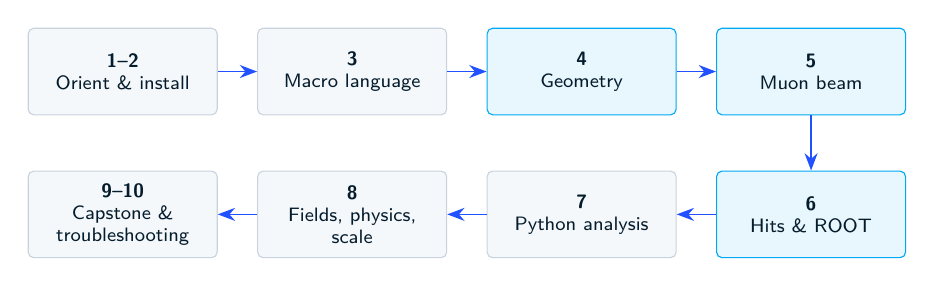
\begin{tikzpicture}[node distance=5mm and 5mm]
  \node[box] (a) {\textbf{1--2}\\Orient \& install};
  \node[box,right=of a] (b) {\textbf{3}\\Macro language};
  \node[hot,right=of b] (c) {\textbf{4}\\Geometry};
  \node[hot,right=of c] (d) {\textbf{5}\\Muon beam};
  \node[hot,below=7mm of d] (e) {\textbf{6}\\Hits \& ROOT};
  \node[box,left=of e] (f) {\textbf{7}\\Python analysis};
  \node[box,left=of f] (g) {\textbf{8}\\Fields, physics,\\scale};
  \node[box,left=of g] (h) {\textbf{9--10}\\Capstone \&\\troubleshooting};
  \draw[arr] (a)--(b); \draw[arr] (b)--(c); \draw[arr] (c)--(d); \draw[arr] (d)--(e);
  \draw[arr] (e)--(f); \draw[arr] (f)--(g); \draw[arr] (g)--(h);
\end{tikzpicture}
\end{center}
{\small\color{muted}Shaded = the core craft. If you only have an afternoon, do Chapters 2, 3, 4 and 6.\par}

\eyebrow{How to read the callouts}
\begin{keypoint}The one idea on the page that, if you remember nothing else, you should remember.\end{keypoint}
\begin{tip}A shortcut, a good habit, or a small trick that saves you time.\end{tip}
\begin{pitfall}A mistake beginners actually make. Read these --- they are the errors that cost an afternoon.\end{pitfall}
\begin{physics}The physics behind the code: why the numbers come out the way they do.\end{physics}
\begin{hood}What Geant4 or \musrSim\ is doing internally. Optional on a first read, useful when debugging.\end{hood}
\begin{checkbuild}Something that may differ in your fork. A prompt to verify against your own source, not to trust blindly.\end{checkbuild}

\eyebrow{Conventions for code}
Shell commands, macro files (\code{.mac}), C++ and Python are shown in monospaced blocks with a blue rule on the left and a caption underneath. A long line that does not fit is wrapped and marked with \(\hookrightarrow\); type it as \emph{one} line. Comments begin with \code{#}. Paths such as \code{build/run} are relative to the top of the repository.

\begin{pitfall}
The single most important convention in this book. In every \code{/musr/command construct} line, box and tube dimensions are \emph{half-lengths}, following Geant4's \code{G4Box} and \code{G4Tubs}. A ``\code{100 100 5}'' box is \(200\times200\times10\)\,mm. Beginners routinely build detectors twice the size they intended. We flag this again in Chapter~\ref{ch:geometry}, but internalise it now.
\end{pitfall}

{\hypersetup{linkcolor=ink}\tableofcontents}


\cleardoublepage
\pagenumbering{arabic}
\chapter{The big picture: what \musrSim\ is}
\label{ch:big}

\begin{willdo}
\begin{itemize}
  \item See where \musrSim\ sits on top of Geant4, and why that matters.
  \item Understand the ``configure in text, run once'' philosophy that shapes everything else.
  \item Walk through the life of a single simulated event, from a command to a number on disk.
  \item Meet the muon physics that makes this toolkit special.
\end{itemize}
\end{willdo}

A muon detector is expensive, slow to build, and unforgiving of mistakes. A simulation is none of those things. Before you cut a single scintillator or book a beamline shift, you can build the whole apparatus in software, fire millions of muons at it, and read out exactly what each counter would see. That is what \musrSim\ is for. This chapter is the map; the rest of the book is the territory.

\section{Geant4, in one paragraph}
Geant4 (``GEometry ANd Tracking'') is a Monte-Carlo toolkit for simulating how particles move through matter. It is developed by an international collaboration --- CERN, KEK, SLAC and many universities --- and is the standard tool across particle, nuclear, medical and space physics. Given a geometry, a set of physics processes and some primary particles, Geant4 transports each particle step by step, deciding at every step whether it scatters, loses energy, decays or creates secondaries, and records what happens.

\begin{hood}
Geant4 is a C++ \emph{library}, not a program. Normally you write C++ classes for your detector, your primary particles and your run logic, compile them against Geant4, and run the result. \musrSim\ is one such program --- written once, so that you don't have to.
\end{hood}

\section{What \musrSim\ adds}
\musrSim\ is a Geant4 application originally written at PSI by K.~Sedlak and colleagues for muon-spin-rotation (\muSR) instruments and beamlines, and since forked and extended by many groups. Its central design choice is this: \emph{you should not have to write or compile C++ to run a new experiment.} The detector geometry, the muon beam, the physics processes and the output are all defined in a plain-text \emph{macro} file. One compiled executable serves every setup.

\begin{keypoint}
\musrSim\ is not a separate simulation engine. It \emph{is} Geant4, pre-wrapped with muon physics and a text-driven geometry builder. Everything you learn here is transferable Geant4 knowledge; \musrSim\ just spares you the boilerplate.
\end{keypoint}

Concretely, \musrSim\ gives you:
\begin{itemize}
  \item a library of ready-made solids you place from the macro (\code{box}, \code{tubs}, \code{cons}, \code{sphere}, and many composite shapes for real spectrometers);
  \item a muon-tuned physics list whose electromagnetic processes you switch on line by line, with muon decay \emph{with spin}, muonium formation and \(\mu^-\) capture available;
  \item a muon-beam generator (\code{/gun/...}) that models beam position, momentum spread, tilt and --- crucially for \muSR\ --- spin polarisation, plus built-in cosmic-ray generators (EcoMug, CRY) for muography;
  \item a ROOT output tree with one row per event.
\end{itemize}

\section{The three layers}
It helps to picture three layers stacked on top of each other. You write the top layer; the bottom two do the work.

\begin{center}
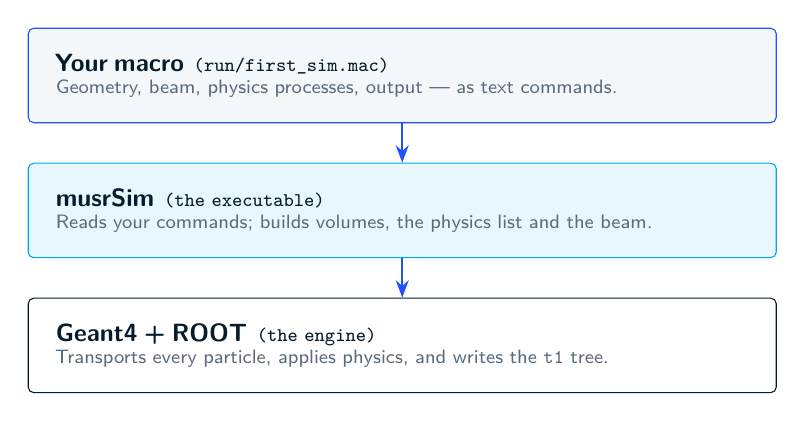
\begin{tikzpicture}[layer/.style={draw=#1,fill=icebg,rounded corners=2pt,minimum width=95mm,minimum height=12mm,align=left,text width=88mm,font=\sffamily\scriptsize,text=muted}]
  \node[layer=eblue] (m) {{\small\bfseries\color{navy}Your macro}\enspace{\ttfamily\color{navy}(run/first\_sim.mac)}\\Geometry, beam, physics processes, output --- as text commands.};
  \node[layer=cyan,fill=cyanbg,below=5mm of m] (e) {{\small\bfseries\color{navy}musrSim}\enspace{\ttfamily\color{navy}(the executable)}\\Reads your commands; builds volumes, the physics list and the beam.};
  \node[layer=navy,fill=white,below=5mm of e] (g) {{\small\bfseries\color{navy}Geant4 + ROOT}\enspace{\ttfamily\color{navy}(the engine)}\\Transports every particle, applies physics, and writes the \texttt{t1} tree.};
  \draw[arr] (m)--(e); \draw[arr] (e)--(g);
\end{tikzpicture}
\end{center}

When you run \code{../musrSim first_sim.mac}, the executable builds the geometry and physics from your macro, then executes the macro's remaining commands --- the beam settings and finally \code{/run/beamOn}, which hands control to Geant4 to simulate the events and fill the ROOT file. You never touch the bottom two layers, but knowing they are there tells you where to look when something behaves oddly.

\section{The life of one event}
Every simulation, no matter how elaborate, follows the same loop. Fixing this picture in your head now will make Chapters~\ref{ch:macro}--\ref{ch:output} feel like variations on a theme rather than a pile of new commands.

\begin{center}
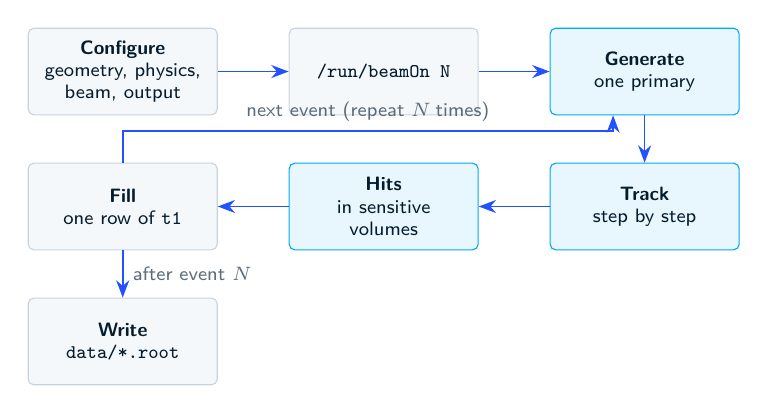
\begin{tikzpicture}[node distance=6mm and 9mm]
  \node[box] (cfg) {\textbf{Configure}\\geometry, physics,\\beam, output};
  \node[box,right=of cfg] (on) {\texttt{/run/beamOn N}};
  \node[hot,right=of on] (gen) {\textbf{Generate}\\one primary};
  \node[hot,below=of gen] (trk) {\textbf{Track}\\step by step};
  \node[hot,left=of trk] (hit) {\textbf{Hits}\\in sensitive\\volumes};
  \node[box,left=of hit] (fill) {\textbf{Fill}\\one row of \texttt{t1}};
  \node[box,below=of fill] (wr) {\textbf{Write}\\\texttt{data/*.root}};
  \draw[arr] (cfg)--(on); \draw[arr] (on)--(gen); \draw[arr] (gen)--(trk);
  \draw[arr] (trk)--(hit); \draw[arr] (hit)--(fill);
  \draw[arr] (fill.north) -- ++(0,4mm) -| node[pos=0.25,above,font=\sffamily\scriptsize,text=muted]{next event (repeat \(N\) times)} ([xshift=-4mm]gen.south) ;
  \draw[arr] (fill)--node[right,font=\sffamily\scriptsize,text=muted]{after event \(N\)}(wr);
\end{tikzpicture}
\end{center}

\begin{keypoint}
An \emph{event} in \musrSim\ is one primary particle (or, for CRY, one cosmic-ray shower) generated and tracked until it and all its secondaries leave the world or stop, with every energy deposit in a sensitive volume recorded as a \emph{hit}. One stored event becomes one row in the output tree.
\end{keypoint}

\begin{pitfall}
Unlike bare Geant4 tutorials, \musrSim\ macros do \emph{not} call \code{/run/initialize}. The executable initialises Geant4 itself, before your macro's commands are executed (Section~\ref{sec:tworeads} explains how). If you copied \code{/run/initialize} from a generic Geant4 example, remove it.
\end{pitfall}

\section{Why muons, and why this toolkit}
Muons are heavy cousins of the electron (\(m_\mu\approx207\,m_e\)), created abundantly in cosmic-ray showers and at accelerator beamlines. Two properties make them uniquely useful, and \musrSim\ is built around both.

\begin{physics}
\textbf{Muons barely notice matter.} A minimum-ionising muon loses only about \SI{2}{MeV} per \si{g.cm^{-2}}, so it punches through metres of rock or metal in a nearly straight line. This is what makes muon radiography (``muography'') possible --- and what lets a few scintillator slabs act as a cosmic-ray telescope.
\end{physics}

\begin{physics}
\textbf{Muons carry a spin you can read.} A polarised muon's spin precesses in a magnetic field, and its direction is imprinted on the direction of the decay positron (\(\mu^+\to e^+\nu_e\bar\nu_\mu\)). Measuring where the positron goes measures the field the muon sat in --- the basis of \muSR. This is why \musrSim\ tracks muon polarisation (the \code{/gun/muonPolariz...} commands and the \code{muDecayPol...} branches) when most toolkits ignore spin entirely.
\end{physics}

The muon's mean lifetime, \(\tau_\mu=\SI{2.197}{\micro s}\), is short enough to measure on a benchtop and long enough that a stopped muon lives well past the prompt flash --- a fact we exploit in Chapters~\ref{ch:python} and~\ref{ch:capstone}.

\section{What you will build in this book}
By Chapter~\ref{ch:capstone} you will have written, run and analysed a complete transverse-field \muSR\ measurement: polarised muons stopping in a copper sample inside a \SI{10}{mT} field, their spins precessing, and two positron counters recording an oscillating asymmetry. Fitting it recovers the field you set --- in our reference run, \SI{9.983(15)}{mT} --- end to end, from a text file to a physics result.

\begin{recap}
\begin{itemize}
  \item \musrSim\ is a text-driven Geant4 application; you configure in a macro and never compile.
  \item Three layers: your macro \(\rightarrow\) \musrSim\ \(\rightarrow\) Geant4/ROOT.
  \item Every event follows the same loop: generate \(\rightarrow\) track \(\rightarrow\) hits \(\rightarrow\) one tree row.
  \item \musrSim\ exists because muons are penetrating and spin-polarised --- it tracks both.
\end{itemize}
\end{recap}
\nextchap{install \musrSim\ and see first light}

\chapter{Installation and first light}
\label{ch:install}

\begin{willdo}
\begin{itemize}
  \item Install the dependencies: Geant4, ROOT, CMake and a C++ compiler.
  \item Get the \texttt{musrSim-upgrade} source and build the \musrSim\ executable.
  \item Run the bundled \code{101.mac} and confirm you get a ROOT file.
  \item Look at the geometry in a 3-D viewer.
\end{itemize}
\end{willdo}

\section{What you need}
{\tablestyle
\begin{tabularx}{\textwidth}{@{}l l L@{}}
\toprule
\textbf{Component} & \textbf{Version} & \textbf{Role}\\
\midrule
Geant4 & 11.x (tested 11.4.3); 10.7 also works & Particle transport engine \\
ROOT & 6.x (tested 6.40) & Output format and C++ analysis \\
CMake & \(\ge\) 3.16 (CMake 4 is fine) & Build system \\
C++ compiler & GCC \(\ge\) 9 or Clang \(\ge\) 12 & C++17 or newer --- the build follows ROOT's standard \\
Python (analysis) & \(\ge\) 3.9 & \code{uproot}, \code{awkward}, \code{numpy}, \code{scipy}, \code{matplotlib} \\
\bottomrule
\end{tabularx}}

\section{The fastest path: one conda environment}
\label{sec:conda}
conda-forge ships Geant4 (with its data sets), ROOT, CMake and a compiler as one consistent set. This is how the reference runs in this book were made:

\begin{lstlisting}[style=sh,caption={Geant4 + ROOT + toolchain from conda-forge (use \texttt{mamba} or \texttt{micromamba} the same way)}]
conda create -n musrsim -c conda-forge geant4 root cmake make cxx-compiler expat
conda activate musrsim
geant4-config --version      # e.g. 11.4.3
root-config --version        # e.g. 6.40.04
\end{lstlisting}

Activating the environment also sets the Geant4 data-set variables, so there is nothing else to source. Add the Python analysis packages to the same environment (Chapter~\ref{ch:python}):

\begin{lstlisting}[style=sh,caption={Analysis packages}]
pip install uproot awkward numpy scipy matplotlib
\end{lstlisting}

\begin{tip}
On a cluster with CVMFS you can skip installing anything: source a CERN LCG view that bundles Geant4, ROOT and a compiler, for example \code{source /cvmfs/sft.cern.ch/lcg/views/LCG_101/x86_64-centos7-gcc11-opt/setup.sh}. Pick a newer LCG release if your site has one.
\end{tip}

\section{Installing the dependencies yourself}
\subsection{Linux (Ubuntu/Debian)}
Install the system libraries Geant4 needs, then build Geant4 from source. ROOT is easiest from the official binaries at \url{root.cern/install}.

\begin{lstlisting}[style=sh,caption={System build dependencies}]
sudo apt-get update
sudo apt-get install -y build-essential cmake \
     libxerces-c-dev libexpat1-dev \
     libgl1-mesa-dev libglu1-mesa-dev libxmu-dev libxi-dev \
     qt6-base-dev
\end{lstlisting}

\begin{lstlisting}[style=sh,caption={Build Geant4 11 from source}]
# after downloading and unpacking geant4-v11.x from geant4.web.cern.ch:
cd geant4-v11.4.3
mkdir build && cd build
cmake -DCMAKE_INSTALL_PREFIX=$HOME/geant4-install \
      -DGEANT4_USE_OPENGL_X11=ON -DGEANT4_USE_QT=ON \
      -DGEANT4_INSTALL_DATA=ON ..
make -j$(nproc)
make install
\end{lstlisting}

\begin{pitfall}
Note \code{mkdir build && cd build} --- the \code{&&} chains the two commands. Writing ``\code{mkdir build} and \code{cd build}'' is not shell syntax. This is a real error we have seen copied from notes.
\end{pitfall}

\subsection{macOS}
ROOT and the build tools come from Homebrew; Geant4 is not in Homebrew core, so build it from source as above --- or simply use the conda environment of Section~\ref{sec:conda}, which works the same on macOS.

\begin{lstlisting}[style=sh,caption={macOS: tools via Homebrew, Geant4 from source}]
brew install cmake root xerces-c qt
# then build Geant4 11 from source as in the Linux section
\end{lstlisting}

\subsection{Make the environments available}
For a self-built toolchain, add these to your \code{~/.bashrc} or \code{~/.zshrc}:

\begin{lstlisting}[style=sh,caption={Shell environment for a self-built Geant4 and a ROOT binary}]
source $HOME/geant4-install/bin/geant4.sh    # Geant4 libraries + data sets
source /path/to/root/bin/thisroot.sh         # ROOT
\end{lstlisting}

\begin{pitfall}
There is no \code{geant4} command and no \code{geant4 --version}. Geant4 exposes its settings through \code{geant4-config} (CMake uses it to find the libraries). If \code{geant4-config} is not found, the environment is not set up.
\end{pitfall}

\section{Get and build \musrSim}
\begin{lstlisting}[style=sh,caption={Clone and build \texttt{musrSim-upgrade}}]
git clone https://github.com/kimsiang/musrSim-upgrade.git
cd musrSim-upgrade
mkdir build
cd build
cmake ../        # finds Geant4 and ROOT from your environment
make -j4         # produces the executable build/musrSim
\end{lstlisting}

\code{cmake} also copies every file in \code{run/} --- the example macros, field maps and setup files --- into \code{build/run/}, which is where you run from. If you edit a macro in \code{run/}, re-run \code{cmake ../} (or simply edit the copy in \code{build/run/}).

\begin{tip}
Build out of source: a separate \code{build/} directory keeps generated files away from the code, so \code{git status} stays clean and \code{rm -rf build} always gives you a fresh start.
\end{tip}

\section{First light: run the bundled example}
\begin{lstlisting}[style=sh,caption={Run your first simulation}]
cd run           # i.e. build/run
mkdir data       # output goes to data/ ; it must exist!
../musrSim 101.mac
\end{lstlisting}

You will see Geant4 print its banners, the physics processes being defined, the list of volumes with overlap checks, and finally a summary like \code{Number of events = 5}. The run writes \code{data/musrSim_jp101.root}.

\begin{keypoint}
Output goes to \code{data/musrSim_jp<NNN>[_<name>].root}, where \code{<NNN>} is the leading integer of the macro's file name, zero-padded to three digits (\code{101.mac} \(\rightarrow\) \code{jp101}; \code{first_sim.mac} has no number \(\rightarrow\) \code{jp000}). The \code{data/} directory must already exist: without it the run stops with \code{!!!FATAL!!! ... Root output file ... can not be created}.
\end{keypoint}

\begin{hood}
The command line is \code{musrSim <macro> [name|idle] [seedOffset]}. Argument~1 is the macro. Argument~2, if given, becomes the \code{_<name>} suffix of the output file --- except the special word \code{idle}, which instead drops you into an interactive Geant4 prompt once the macro has finished. Argument~3 is a random-seed offset for batch jobs (Section~\ref{sec:scale}). Run without arguments, \musrSim\ only prints this usage line.
\end{hood}

\code{101.mac} simulates five muons and stores only events with a hit in detector~11, so its tree holds a single entry --- enough to prove the chain works. Chapter~\ref{ch:macro} builds a macro of your own.

\section{See the geometry}
A simulation you cannot see is a simulation you cannot trust. The repository ships visualisation macros you call from inside a steering macro, just before \code{/run/beamOn}:

\begin{lstlisting}[style=mac,caption={Write a VRML scene of the geometry and the first trajectories}]
/control/execute visVRML.mac
/run/beamOn 5
\end{lstlisting}

\code{visVRML.mac} opens Geant4's \code{VRML2FILE} driver, which writes \code{g4_00.wrl} (one file per run) for any VRML viewer. For a live OpenGL or Qt window instead, copy it and change its first line to \code{/vis/open OGL} or \code{/vis/open TSG_QT_GLES}; this needs a Geant4 built with those drivers. Keep \code{/run/beamOn} small whenever visualisation is on --- every trajectory is stored. We return to visualisation in Chapter~\ref{ch:geometry}.

\section{Troubleshooting the build}
{\tablestyle
\begin{tabularx}{\textwidth}{@{}>{\raggedright\arraybackslash}p{0.38\textwidth} L@{}}
\toprule
\textbf{Symptom} & \textbf{Fix}\\
\midrule
\code{Could NOT find Geant4} & Activate the conda environment or source \code{geant4.sh}; or pass \code{-DGeant4_DIR=<prefix>/lib/cmake/Geant4}.\\
\code{root-config} not found & Source \code{thisroot.sh} (or activate the environment) before \code{cmake}; \musrSim\ finds ROOT through \code{root-config}.\\
\code{Could NOT find EXPAT: Found unsuitable version} & CMake picked up an old system \code{libexpat}. Install \code{expat} in the conda environment and configure with \code{cmake -DCMAKE_PREFIX_PATH=$CONDA_PREFIX ../}.\\
Compile errors about missing Geant4 classes & You are on a fork older than \texttt{musrSim-upgrade}; pull the current code, which builds on Geant4 10.7--11.x.\\
Runs, but stops with \code{Root output file ... can not be created} & The \code{data/} directory does not exist where you launched. \code{mkdir data}.\\
Viewer window never opens & Your Geant4 was built without OpenGL/Qt; use \code{visVRML.mac}, or rebuild Geant4 with \code{-DGEANT4_USE_QT=ON}.\\
\bottomrule
\end{tabularx}}

\begin{recap}
\begin{itemize}
  \item One conda-forge environment gives a matching Geant4 + ROOT + compiler; CVMFS gives it for free on clusters.
  \item Build out of source: \code{cmake ../} then \code{make -j4} produces \code{build/musrSim} and copies \code{run/} to \code{build/run/}.
  \item Run \code{../musrSim <macro>} from \code{build/run}; create \code{data/} first; output is \code{data/musrSim_jp<NNN>.root}.
  \item \code{/control/execute visVRML.mac} before \code{/run/beamOn} gives you a 3-D picture.
\end{itemize}
\end{recap}
\nextchap{the macro language, and your first macro from scratch}

\chapter{The macro language, and your first simulation}
\label{ch:macro}

\begin{willdo}
\begin{itemize}
  \item Recognise the three families of commands a \musrSim\ macro is built from.
  \item Understand the two ways \musrSim\ reads your macro --- the key to every ``why was my line ignored?''.
  \item List the commands your executable understands.
  \item Write, run and inspect a complete simulation from a blank file.
\end{itemize}
\end{willdo}

A \musrSim\ macro (also called the \emph{steering file}) is a plain-text script. There is no compilation step: change a number, run again. Master this one file and you can build almost any instrument without touching C++.

\section{Three families of commands}
Every line in a working macro belongs to one of three families. Telling them apart is the single most useful orientation skill in this toolkit.

{\tablestyle
\begin{tabularx}{\textwidth}{@{}>{\raggedright\arraybackslash}p{0.22\textwidth} >{\raggedright\arraybackslash}p{0.27\textwidth} L@{}}
\toprule
\textbf{Family} & \textbf{Prefix} & \textbf{What it controls}\\
\midrule
Standard Geant4 & \code{/run}, \code{/vis}, \code{/tracking}, \code{/control}, \code{/process}, \code{/gps} & Universal Geant4 kernel commands, identical in every Geant4 application.\\
\musrSim\ core & \code{/musr/command} & Geometry, fields, physics processes, output selection. Read directly from the file by \musrSim's C++ (next section).\\
\musrSim\ run control & \code{/musr/run} & Random seeding, progress printout.\\
Beam (particle gun) & \code{/gun} & The muon beam model: vertex, momentum, spin, decay timing, TURTLE input, and the cosmic-ray generators.\\
\bottomrule
\end{tabularx}}

\begin{keypoint}
The \code{/run}, \code{/vis} and \code{/control} commands are documented in the official Geant4 guides and never change. The \code{/musr/...} and \code{/gun/...} commands are the ones this book teaches, because they live in your copy of the source and differ between forks. When in doubt about a \musrSim-specific command, the source is the specification.
\end{keypoint}

\section{How \musrSim\ reads a macro: twice}
\label{sec:tworeads}
This is the one piece of plumbing worth understanding before you write a line. Your macro is read in two different ways.

\begin{center}
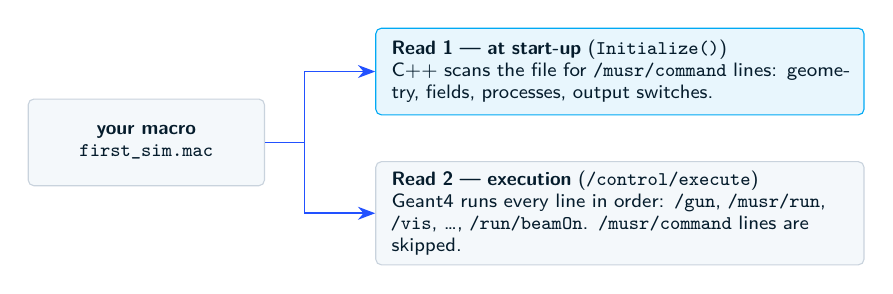
\begin{tikzpicture}[node distance=4mm and 8mm]
  \node[box,minimum width=30mm] (file) {\textbf{your macro}\\\texttt{first\_sim.mac}};
  \node[hot,right=14mm of file,yshift=9mm,minimum width=62mm,align=left,text width=58mm] (r1) {\textbf{Read 1 --- at start-up} (\texttt{Initialize()})\\C++ scans the file for \texttt{/musr/command} lines: geometry, fields, processes, output switches.};
  \node[box,right=14mm of file,yshift=-9mm,minimum width=62mm,align=left,text width=58mm] (r2) {\textbf{Read 2 --- execution} (\texttt{/control/execute})\\Geant4 runs every line in order: \texttt{/gun}, \texttt{/musr/run}, \texttt{/vis}, \dots, \texttt{/run/beamOn}. \texttt{/musr/command} lines are skipped.};
  \draw[arr] (file.east) -- ++(5mm,0) |- (r1.west);
  \draw[arr] (file.east) -- ++(5mm,0) |- (r2.west);
\end{tikzpicture}
\end{center}

\textbf{Read 1 --- start-up.} \code{main()} first creates the detector and the physics list and calls Geant4's \code{Initialize()}. During that call \code{musrDetectorConstruction} and \code{musrPhysicsList} each open your macro \emph{as a text file} and parse every line that starts with \code{/musr/command}, top to bottom: volumes, rotations, fields, \code{rootOutput} switches, \code{process} lines.

\textbf{Read 2 --- execution.} Only then does \code{main()} run \code{/control/execute <yourfile>}. Now Geant4 executes the macro line by line as ordinary UI commands: \code{/gun/...} sets the beam, \code{/musr/run/...} sets seeding, \code{/vis/...} sets up pictures, and \code{/run/beamOn} starts the events. The \code{/musr/command} lines are passed to a messenger that deliberately ignores them --- they have already done their job.

Three practical rules follow.
\begin{enumerate}
  \item \textbf{No \code{/run/initialize}.} Initialisation has already happened before Read~2 begins; your macro simply ends with \code{/run/beamOn}.
  \item \textbf{Order matters among \code{/musr/command} lines}: a mother volume before its daughters, a rotation matrix before the volume that uses it, a volume before the field attached to it. Where they sit relative to \code{/gun} lines does not matter.
  \item \textbf{\code{/musr/command} lines must be in the macro you pass on the command line.} Read~1 does not follow \code{/control/execute}, so geometry or physics in an included file is silently never built. Included files are fine for \code{/vis} and \code{/gun} commands --- that is exactly how \code{visVRML.mac} works.
\end{enumerate}

\begin{hood}
You can see both reads in \code{musrSim.cc}: \code{runManager->Initialize()} comes first, then \code{UI->ApplyCommand("/control/execute " + fileName)}. The parsing loops are \code{musrDetectorConstruction::Construct()} and \code{musrPhysicsList::ConstructEM()}; both skip lines whose first character is \code{#}.
\end{hood}

\section{List the real commands}
\label{sec:listcommands}
Before trusting any command in any manual --- including this one --- ask your executable what it supports. Run any macro with \code{idle} as the second argument: once the macro has finished you get Geant4's \code{Idle>} prompt, where you can browse the live command tree.

\begin{lstlisting}[style=sh,caption={Discovering \texttt{/gun} and \texttt{/musr/run} commands without reading C++}]
cd build/run
../musrSim first_sim.mac idle
# at the Idle> prompt:
#   ls /gun/                       list every beam command (and /gun/cry/, /gun/ecomug/)
#   help /gun/decaytimelimits      one command's parameters and guidance
#   ls /musr/run/                  seeding and printout commands
#   /control/manual /gun/          dump a whole subtree as text
#   exit
\end{lstlisting}

\code{ls} walks the command tree one level at a time; \code{help <command>} prints the parameters and the author's own description straight from the code; \code{/control/manual} dumps a subtree, which you can paste into your notes as a personal, always-correct reference.

\begin{checkbuild}
\code{/musr/command} is a \emph{single} UI command that takes the rest of the line as a string, so \code{ls} cannot show its keywords (\code{construct}, \code{globalfield}, \dots). Those are \code{strcmp} branches in the C++ parsers. Appendix~\ref{app:commands} lists every keyword in this build, and Section~\ref{sec:rejected} shows how to look one up in the source.
\end{checkbuild}

\section{Comments and units}
Lines beginning with \code{#} are comments. Keep comments on their own lines: the Geant4 UI strips a trailing \code{# ...}, but \musrSim's own parsers read \code{/musr/command} lines with fixed field positions, and a stray word can be mistaken for a value.

Inside \code{/musr/command} lines the units are fixed: millimetres, degrees, tesla, nanoseconds. \code{/gun} commands accept an explicit unit and you should always give one: \code{/gun/momentum 29.8 MeV}, \code{/gun/vertex 0 0 -100 mm}. Being explicit in the beam block costs nothing and prevents a factor-of-ten surprise.

\section{Your first macro, from a blank file}
\label{sec:firstmacro}
Here is a complete, self-contained simulation: a box of air (the mandatory \code{World}), one plastic-scintillator slab wired up as a detector, the electromagnetic physics, a small surface-muon beam aimed at the slab, and a line telling \musrSim\ to keep only events that hit something. It ships as \code{run/first_sim.mac}.

\lstinputlisting[style=mac,caption={\texttt{first\_sim.mac} --- a minimal but complete simulation},label=lst:firstsim]{../run/first_sim.mac}

The geometry is two lines. The \code{World} is a \SI{1}{m} cube of air (half-lengths \SI{500}{mm}); the mother of the world is the literal token \code{no_logical_volume}. The \code{Slab} is a \(100\times100\times\SI{10}{mm}\) block of plastic scintillator at the origin, made sensitive by the token \code{musr/ScintSD} and given detector ID~1. The middle block switches on the physics, and the rest is beam and bookkeeping, which the next chapters unpack in full.

\subsection{The physics block}
\label{sec:physicsblock}
\begin{pitfall}
\musrSim\ builds its electromagnetic physics \emph{from your macro}. Without the \code{/musr/command process} lines, photons, electrons, positrons and muons have no ionisation, scattering or annihilation at all: muons sail straight through the slab, nothing deposits energy, and the output tree is empty. We checked: \code{first_sim.mac} with the physics block removed stores \textbf{zero} of 20\,000 events. Copy the block from \code{first_sim.mac} into every new macro.
\end{pitfall}

Each \code{addProcess} line names a particle, a Geant4 process class and three ordering numbers (at-rest, along-step, post-step; \code{-1} means ``not active''). Muon decay \emph{with spin} is added automatically for \(\mu^\pm\); everything else is your choice. Section~\ref{sec:physics} lists the processes you can add.

\subsection{Run it}
\begin{lstlisting}[style=sh,caption={Run your first macro}]
cd build/run
mkdir -p data
../musrSim first_sim.mac      # run number 0: the file name has no leading integer
ls -l data/                   # -> musrSim_jp000.root
\end{lstlisting}

In our reference run 19\,991 of the 20\,000 events were stored; the handful of others left no hit and were dropped by \code{storeOnlyEventsWithHits}. The muons stop about \SI{0.8}{mm} inside the slab's front face and decay there.

\begin{pitfall}
Three first-run failures, and their fixes. \emph{The run stops with ``can not be created''} --- you forgot \code{mkdir -p data}. \emph{An empty tree} --- the physics block is missing, or nothing reaches your sensitive volume. \emph{The slab is twice too big} --- you typed full lengths where Geant4 wants \emph{half}-lengths (Chapter~\ref{ch:geometry} hammers this home).
\end{pitfall}

\begin{physics}
Surface muons carry a momentum near \SI{29.8}{MeV/c} (kinetic energy \(\approx\)\,\SI{4.1}{MeV}) and are almost \SI{100}{\percent} spin-polarised \emph{anti-parallel} to their momentum --- the property that makes muon spin spectroscopy possible. That is why a beam travelling along \(+z\) is paired with \code{/gun/muonPolarizVector 0 0 -1}. We return to the spin in Chapter~\ref{ch:beam}.
\end{physics}

To peek at the result before building the analysis toolchain (Chapters~\ref{ch:output}--\ref{ch:python}), open the file in ROOT:

\begin{lstlisting}[style=cpp,caption={A first look with ROOT}]
root -l data/musrSim_jp000.root
root [0] t1->Print()                 // list every branch in the tree
root [1] t1->Draw("det_edep")        // energy deposited per hit (MeV)
root [2] t1->Draw("muDecayTime")     // when each muon decayed (microseconds)
root [3] .q
\end{lstlisting}

\begin{figure}[h]
\centering
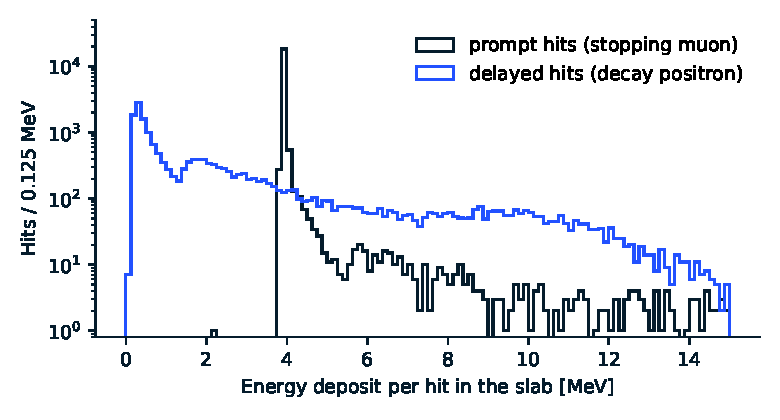
\includegraphics[width=0.78\textwidth]{figures/edep_spectrum.pdf}
\caption{Energy per hit in the slab, from the reference run of \texttt{first\_sim.mac} (log scale). Each muon produces two hits: a \emph{prompt} one as it stops, depositing its full \(\approx\)\SI{4}{MeV} kinetic energy (sharp peak), and a \emph{delayed} one, microseconds later, from its decay positron (broad spectrum). Muons that decay within the \SI{100}{ns} hit-separation window merge both into one prompt hit --- the prompt tail above \SI{4}{MeV}.}
\label{fig:edep}
\end{figure}

\begin{recap}
\begin{itemize}
  \item Macros mix universal Geant4 commands, \musrSim's \code{/musr/command} and \code{/musr/run}, and the \code{/gun} beam.
  \item \code{/musr/command} lines are parsed from the file at start-up; everything else is executed in order afterwards. No \code{/run/initialize}; no \code{/musr/command} in included files.
  \item \code{../musrSim macro.mac idle} gives you a prompt where \code{ls} and \code{help} list the real \code{/gun} and \code{/musr/run} commands.
  \item A complete simulation needs a \code{World}, one sensitive volume, \emph{the physics block}, a beam, and \code{/run/beamOn}.
\end{itemize}
\end{recap}
\nextchap{building real geometry with the \texttt{construct} command}

\chapter{Building geometry with \texttt{construct}}
\label{ch:geometry}

\begin{willdo}
\begin{itemize}
  \item Read and write the \code{/musr/command construct} line field by field.
  \item Never again confuse a half-length with a length.
  \item Nest volumes correctly using the \code{log_} mother convention and local coordinates.
  \item Rotate volumes, choose materials, import CAD, make a volume a detector, and use the special volume names.
\end{itemize}
\end{willdo}

Almost all of an instrument is geometry, and in \musrSim\ almost all geometry is one command repeated: \code{/musr/command construct}. Each call builds one Geant4 volume --- a shape, made of a material, placed inside a parent. Learn this single line thoroughly and the rest is repetition.

\section{The construct grammar}
Every \code{construct} call has the same field order. Here is the world volume from the bundled GPD example, \code{run/201.mac}, with each field numbered.

\begin{lstlisting}[style=mac,caption={One \texttt{construct} line, dissected}]
/musr/command construct box World 2100 2100 11000 G4_AIR 0 0 0 no_logical_volume norot dead -1
#                       (1)  (2)  (3)--------------(4)    (5)-- (6)-------------- (7)-- (8)-(9)
\end{lstlisting}

\begin{enumerate}[label=\textbf{(\arabic*)}]
  \item \textbf{solid} --- the shape keyword: \code{box}, \code{tubs}, \code{cons}, \code{sphere}, \code{trd}, \code{para}, \code{torus}, \code{polyconeA}/\code{polyconeB}, \code{stl}, or a composite shape hard-coded in the source (Section~\ref{sec:solids}).
  \item \textbf{name} --- your label for this volume. Its logical volume is then referred to elsewhere as \code{log_<name>} (here \code{log_World}). Choose names carefully: some names are magic (Section~\ref{sec:magic}).
  \item \textbf{dimensions} --- the size parameters for that solid, in millimetres and degrees. Their number depends on the shape. For boxes and tubes these are \emph{half}-lengths (Section~\ref{sec:half}).
  \item \textbf{material} --- a Geant4/NIST material such as \code{G4_AIR}, \code{G4_Cu}, \code{G4_Galactic} (vacuum) or \code{G4_PLASTIC_SC_VINYLTOLUENE} (Section~\ref{sec:solids}).
  \item \textbf{x y z} --- the position of this volume's centre, in the local coordinates of its mother, in mm.
  \item \textbf{mother} --- the logical volume that contains this one, written \code{log_<mother>}. The world is the sole exception: its mother is the literal token \code{no_logical_volume}.
  \item \textbf{rotation} --- the name of a rotation matrix defined earlier, or \code{norot} (Section~\ref{sec:rot}).
  \item \textbf{sensitivity} --- \code{musr/ScintSD} to make it a detector, or \code{dead} for inert material (Section~\ref{sec:magic}).
  \item \textbf{volumeID} --- an integer that identifies this volume in the ROOT output. For detectors it becomes \code{det_ID}; for every volume it is the label stored in \code{muDecayDetID} when a muon decays there.
\end{enumerate}

\begin{keypoint}
The world volume must be named exactly \code{World}, must use \code{no_logical_volume} as its mother, and is conventionally \code{dead} with ID \code{-1}. Everything else you build lives inside it, directly or indirectly.
\end{keypoint}

\section{Half-lengths: the number-one beginner trap}
\label{sec:half}
For a box, the three dimensions are the \emph{half}-widths along \(x\), \(y\) and \(z\) --- not the full edge lengths. This is inherited straight from Geant4's \code{G4Box}. The same convention applies to the \(z\)-extent of a \code{tubs} (tube) and to most other solids.

\begin{center}
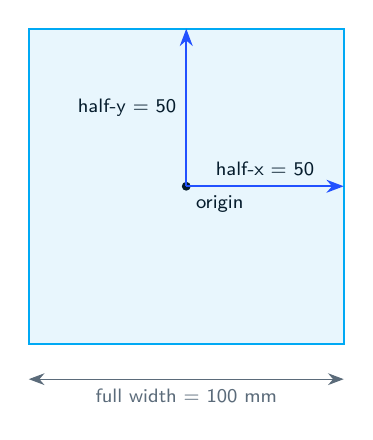
\begin{tikzpicture}[scale=1]
  \draw[fill=cyanbg,draw=cyan,line width=0.8pt] (-2,-2) rectangle (2,2);
  \fill[navy] (0,0) circle (1.6pt) node[below right,font=\sffamily\scriptsize,text=navy]{origin};
  \draw[arr] (0,0) -- (2,0) node[midway,above,font=\sffamily\scriptsize,text=navy]{half-x = 50};
  \draw[arr] (0,0) -- (0,2) node[midway,left,font=\sffamily\scriptsize,text=navy]{half-y = 50};
  \draw[{Stealth[length=2mm]}-{Stealth[length=2mm]},muted] (-2,-2.45) -- (2,-2.45) node[midway,below,font=\sffamily\scriptsize]{full width = 100 mm};
\end{tikzpicture}
\end{center}

So \code{construct box Slab 50 50 5 ...} creates a slab that is \SI{100}{mm} wide, \SI{100}{mm} tall and \SI{10}{mm} thick. If you mean a \SI{100}{mm} cube you write \code{50 50 50}, not \code{100 100 100}.

\begin{pitfall}
Doubling errors from this one convention are the most common geometry bug in Geant4. When a detector seems twice as efficient as it should be, or a collimator hole is half the expected size, check your half-lengths first. A useful habit: write the intended full size in a comment line just above the \code{construct}.
\end{pitfall}

\section{Mothers, daughters, and local coordinates}
Geant4 geometry is a strict hierarchy. Every volume (except the world) sits inside exactly one mother volume, and its position is given in the mother's \emph{local} frame, with the mother's centre as origin. A daughter must fit entirely within its mother, and sibling daughters must not intersect.

\begin{center}
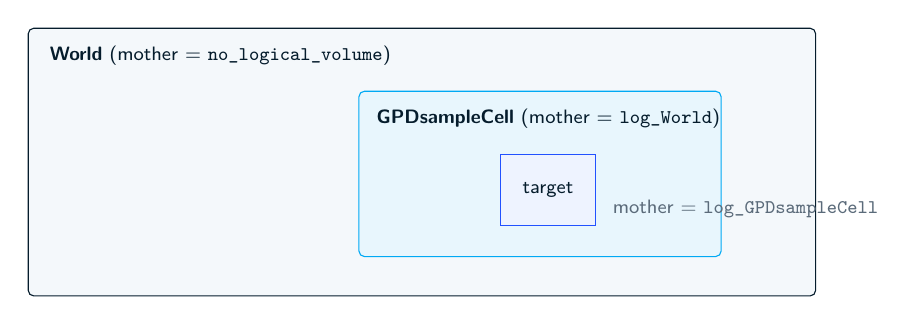
\begin{tikzpicture}
  \draw[draw=navy,fill=icebg,rounded corners=2pt] (0,0) rectangle (10,3.4);
  \node[font=\sffamily\scriptsize,text=navy,anchor=north west] at (0.15,3.3) {\textbf{World} (mother = \texttt{no\_logical\_volume})};
  \draw[draw=cyan,fill=cyanbg,rounded corners=2pt] (4.2,0.5) rectangle (8.8,2.6);
  \node[font=\sffamily\scriptsize,text=navy,anchor=north west] at (4.3,2.5) {\textbf{GPDsampleCell} (mother = \texttt{log\_World})};
  \draw[draw=eblue,fill=paleblue] (6.0,0.9) rectangle (7.2,1.8);
  \node[font=\sffamily\scriptsize,text=navy] at (6.6,1.35) {target};
  \node[font=\sffamily\scriptsize,text=muted,anchor=west] at (7.3,1.1) {mother = \texttt{log\_GPDsampleCell}};
\end{tikzpicture}
\end{center}

To place a volume inside a mother other than the world, set field~(6) to \code{log_<mothername>} and give its coordinates relative to that mother. In \code{201.mac} the copper target sits inside a sample cell, not directly in the world:

\begin{lstlisting}[style=mac,caption={A daughter inside a non-world mother (from \texttt{201.mac})}]
/musr/command construct tubs target 0 3.5 7 0 360 G4_Cu 0 0 0 log_GPDsampleCell norot dead 201
\end{lstlisting}

The target's centre is at \((0,0,0)\) in the sample cell's frame, which itself may sit deep inside the world. You cannot read a volume's global position from its \code{construct} line alone --- follow the chain of mothers.

\begin{pitfall}
The mother must be constructed \emph{before} the daughter, and referenced by its logical name \code{log_<mother>}, not its bare name. Writing \code{GPDsampleCell} instead of \code{log_GPDsampleCell}, or placing the daughter above the mother in the file, stops the run with a ``logical volume not found'' error.
\end{pitfall}

\section{Rotations}
\label{sec:rot}
A volume is placed unrotated with the keyword \code{norot}. To rotate it, first define a named rotation matrix on an earlier line, then use that name in field~(7). \musrSim\ accepts two forms and tells them apart by the fourth number.

\textbf{Axis--angle.} Give a rotation axis \((a_x,a_y,a_z)\) and a non-zero angle in degrees. From \code{201.mac}:

\begin{lstlisting}[style=mac,caption={Axis--angle rotations: axis, then angle}]
# 90 deg about the x-axis; 28.81 deg about y; 45 deg about z
/musr/command rotation matrix1 1 0 0 90
/musr/command rotation matrix2 0 1 0 28.81
/musr/command rotation matrix4 0 0 1 45
\end{lstlisting}

\textbf{Euler angles.} Give three angles \(\phi,\theta,\psi\) in degrees and no fourth number (or a fourth number of zero):

\begin{lstlisting}[style=mac,caption={Euler-angle rotation}]
/musr/command rotation matrix6 180 90 90
\end{lstlisting}

You then attach the matrix by name, exactly as the backward positron counters in \code{201.mac} do:

\begin{lstlisting}[style=mac,caption={Using a named rotation when placing a volume}]
/musr/command construct box ScintB1 13 45 2.5 G4_PLASTIC_SC_VINYLTOLUENE 22 0 -40 log_World matrix2 musr/ScintSD 1
\end{lstlisting}

\begin{tip}
Rotations are easy to get backwards. Define one, place one volume with it, visualise (Section~\ref{sec:seeit}), and confirm the orientation before you build ten more volumes on the same matrix.
\end{tip}

\section{Materials and solids}
\label{sec:solids}
Materials are given by their Geant4/NIST names. You do not define common materials; you name them. The handful you will use constantly:

{\tablestyle
\begin{tabularx}{\textwidth}{@{}>{\raggedright\arraybackslash}p{0.42\textwidth} L@{}}
\toprule
\textbf{NIST name} & \textbf{What it is}\\
\midrule
\code{G4_Galactic} & Ideal vacuum (beam pipes, ``save'' planes).\\
\code{G4_AIR} & Air --- the usual world material.\\
\code{G4_PLASTIC_SC_VINYLTOLUENE} & Plastic scintillator --- muon and positron counters.\\
\code{G4_Cu}, \code{G4_Al}, \code{G4_Pb}, \code{G4_W} & Copper, aluminium, lead, tungsten (samples, holders, collimators).\\
\code{G4_MYLAR}, \code{G4_KAPTON}, \code{G4_POLYETHYLENE} & Windows and light materials.\\
\bottomrule
\end{tabularx}}

About fifty extra materials are defined in \code{musrDetectorConstruction::DefineMaterials()} and used by their bare names: \code{Scintillator}, \code{Mylar}, \code{Brass}, \code{Steel}, \code{Water}, \code{Aerogel}, \code{LaBr3}, \code{Macor}, \code{MgO}, \code{Vacuum}, low-pressure air and helium (\code{Air1mbar}, \code{HeliumGas5mbar}, \dots) and --- for muography --- \code{Rock} and \code{Concrete}. Check that function for the exact compositions before relying on one.

{\tablestyle
\begin{tabularx}{\textwidth}{@{}l >{\raggedright\arraybackslash}p{0.42\textwidth} L@{}}
\toprule
\textbf{Solid} & \textbf{Dimension fields} & \textbf{Notes}\\
\midrule
\code{box} & half-x, half-y, half-z & Rectangular block.\\
\code{tubs} & rMin, rMax, half-z, \(\phi_0\), \(\Delta\phi\) & Cylinder or tube; angles in degrees.\\
\code{cons} & rMin1, rMax1, rMin2, rMax2, half-z, \(\phi_0\), \(\Delta\phi\) & Cone / truncated cone.\\
\code{sphere} & rMin, rMax, \(\phi_0\), \(\Delta\phi\), \(\theta_0\), \(\Delta\theta\) & Full or partial sphere.\\
\code{trd} & half-x1, half-x2, half-y1, half-y2, half-z & Trapezoid.\\
\code{para} & half-x, half-y, half-z, \(\alpha\), \(\theta\), \(\phi\) & Parallelepiped.\\
\code{torus} & rMin, rMax, rTorus, \(\phi_0\), \(\Delta\phi\) & Torus.\\
\code{polyconeA} & \(\phi_0\), \(\Delta\phi\), \(n\), then three array names (z, rInner, rOuter) & Arrays defined with \code{arrayDef}.\\
\code{stl} & a file name instead of dimensions & CAD import (below).\\
\multicolumn{3}{@{}p{\linewidth}@{}}{\small Composite shapes hard-coded in the source: \code{GPDcollimator}, \code{uprofile}, \code{tubsbox}, \code{boxbox}, \code{cruciform}, \dots\ (Appendix~\ref{app:solids}).}\\
\bottomrule
\end{tabularx}}

The beam pipe in \code{201.mac} shows the \code{tubs} field order in practice --- a vacuum cylinder, radius 0 to \SI{2005}{mm}, half-length \SI{4500}{mm}, full azimuth:

\begin{lstlisting}[style=mac,caption={A tube (\texttt{tubs}): rMin rMax half-z phiStart phiTotal}]
/musr/command construct tubs beampipeA 0 2005 4500 0 360 G4_Galactic 0 0 -6100 log_World norot dead 230
\end{lstlisting}

Polycones take their profile from named arrays, defined first with \code{arrayDef <name> <n> <values...>}:

\begin{lstlisting}[style=mac,caption={A polycone from three arrays (from \texttt{201.mac}, shortened to 4 planes)}]
/musr/command arrayDef zPl  4   0.   5.   91.  105.
/musr/command arrayDef rIn  4  10.  11.   31.   31.
/musr/command arrayDef rOut 4  12.5 15.11 35.11 35.
/musr/command construct polyconeA veto 0 360 4 zPl rIn rOut G4_PLASTIC_SC_VINYLTOLUENE 0 0 24 log_World norot musr/ScintSD 51
\end{lstlisting}

\begin{newin}
\textbf{CAD import.} \code{construct stl <name> <file.stl> <material> <x y z> <log_mother> <rotation> <sensitivity> <volumeID>} reads a tessellated solid from an STL file through the bundled CADMesh library --- handy for a real detector housing or a building in a muography study. CADMesh assumes the STL coordinates are in millimetres. Tessellated solids are slow to track through, so keep meshes modest.
\end{newin}

\begin{hood}
Composite solids such as \code{GPDcollimator} exist because Geant4 Boolean operations (subtracting one solid from another) cannot be expressed through the macro grammar. When you need a shape the macro cannot describe, add it to \code{musrDetectorConstruction.cc} and expose it as a new solid keyword --- exactly how \code{GPDcollimator} was created --- or import it with \code{stl}.
\end{hood}

\section{Making a volume a detector, and the magic names}
\label{sec:magic}
Field~(8) decides whether a volume records anything. \code{dead} means inert material that still scatters and stops particles but produces no hits. \code{musr/ScintSD} makes the volume a \emph{sensitive detector}: energy deposits inside it become hits in the ROOT tree, tagged with the integer volumeID you gave in field~(9). That integer appears in the output as \code{det_ID}, and it is how you will later tell one counter from another.

\begin{lstlisting}[style=mac,caption={Five sensitive counters, distinguished only by their volumeID (from \texttt{201.mac})}]
/musr/command construct box ScintB1 13 45 2.5 G4_PLASTIC_SC_VINYLTOLUENE  22 0 -40 log_World matrix2 musr/ScintSD 1
/musr/command construct box ScintB2 13 45 2.5 G4_PLASTIC_SC_VINYLTOLUENE -22 0 -40 log_World matrix3 musr/ScintSD 2
/musr/command construct box ScintF1 13 45 2.5 G4_PLASTIC_SC_VINYLTOLUENE -22 0  40 log_World matrix2 musr/ScintSD 11
/musr/command construct box ScintF2 13 45 2.5 G4_PLASTIC_SC_VINYLTOLUENE  22 0  40 log_World matrix3 musr/ScintSD 12
/musr/command construct box M0 5 5 1.0 G4_PLASTIC_SC_VINYLTOLUENE 0 0 -46 log_World matrix4 musr/ScintSD 102
\end{lstlisting}

\begin{keypoint}
\code{musr/ScintSD} is the sensitive-detector type for energy deposits. You do not create ten detector types; you create ten sensitive volumes, give each a distinct volumeID, and separate them at analysis time by selecting on \code{det_ID}. This is the mental model that makes the ROOT output (Chapter~\ref{ch:output}) click. (A separate optical-photon readout exists for photocathode studies; see Section~\ref{sec:optical}.)
\end{keypoint}

Some names are not just labels --- \musrSim\ treats them specially:

{\tablestyle
\begin{tabularx}{\textwidth}{@{}>{\raggedright\arraybackslash}p{0.28\textwidth} L@{}}
\toprule
\textbf{Name} & \textbf{Special behaviour}\\
\midrule
\code{World} & The mandatory outermost volume; mother is \code{no_logical_volume}.\\
\code{Target} or \code{target} (exact) & Assumed to be the sample. Muon time, polarisation and momentum on entry are stored as \code{muTarget...}; these branches only exist when such a volume is built.\\
\code{M0}, \code{M1}, \code{M2} (exact; or lower-case) & Typically trigger counters. Muon time and polarisation on entry stored as \code{muM0...}, etc.\\
name \emph{containing} \code{save} & A tracking plane: records every particle crossing it (\code{save_...} branches), even in vacuum and with no energy deposit. Give it a non-zero volumeID --- ID~0 is not stored.\\
name \emph{starting with} \code{kill} or \code{Kill} & Any particle entering is deleted from the simulation.\\
name \emph{starting with} \code{shield} or \code{Shield} & Deletes every particle \emph{except muons} --- used to speed up runs by discarding tracks that cannot reach a detector. Use with care.\\
\bottomrule
\end{tabularx}}

\begin{pitfall}
The magic is triggered by the name. A volume you innocently call \code{PbSaver} or \code{savePlate} becomes a tracking plane (``save'' matches anywhere in the name); one you call \code{killswitch} deletes particles. If you do not want the special behaviour, keep these words out of your names.
\end{pitfall}

\section{Seeing it, and checking for overlaps}
\label{sec:seeit}
Colour a logical volume with \code{visattributes} (this only affects visualisation, never physics):

\begin{lstlisting}[style=mac,caption={Colours for visualisation}]
/musr/command visattributes log_World invisible
/musr/command visattributes log_target blue
/musr/command visattributes log_ScintB1 green
\end{lstlisting}

Available colours are \code{invisible}, \code{white}, \code{black}, \code{gray}, \code{red}, \code{darkred}, \code{green}, \code{blue}, \code{lightblue}, \code{darkblue}, \code{cyan}, \code{magenta}, \code{yellow}, \code{oxsteel}, and several house styles (\code{SCINT_style}, \code{MCP_style}, \dots); you may also colour by material name (\code{/musr/command visattributes G4_Cu red}). More can be added in \code{musrDetectorConstruction::SetColourOfLogicalVolume}.

Overlap checking is on in this codebase: every placement is checked as it is created, and the log shows a line \code{Checking overlaps for volume ... OK!} for each. An overlap corrupts particle transport without any other symptom, so never ignore a failed check.

\begin{checkbuild}
If a placement reports an overlap, fix the geometry before trusting a single number from the run. The usual causes are a daughter larger than its mother, a forgotten half-length, or a position that pushes a daughter through a wall. Then look at it: \code{/control/execute visVRML.mac} before \code{/run/beamOn 5} writes a 3-D scene you can rotate in any VRML viewer.
\end{checkbuild}

\begin{recap}
\begin{itemize}
  \item \code{construct} fields, in order: solid, name, dimensions, material, \code{x y z}, \code{log_mother}, rotation, sensitivity, volumeID.
  \item Box and tube dimensions are \emph{half}-lengths; positions are in the mother's local frame.
  \item Rotations are axis--angle (four numbers) or Euler (three), defined before use.
  \item \code{musr/ScintSD} plus a unique volumeID makes a counter; \code{det_ID} separates counters later.
  \item The names \code{Target}, \code{M0}--\code{M2}, \code{*save*}, \code{kill*} and \code{shield*} trigger special behaviour.
\end{itemize}
\end{recap}
\nextchap{the muon beam, its spin, and TURTLE input}

\chapter{The muon beam and its spin}
\label{ch:beam}

\begin{willdo}
\begin{itemize}
  \item Configure the muon beam: species, vertex, spread, momentum and direction.
  \item Set the muon spin --- the quantity that makes muon spin spectroscopy possible.
  \item Control muon decay timing, and feed a realistic beam from a TURTLE file.
  \item Know when to reach for the General Particle Source or a cosmic-ray generator instead.
\end{itemize}
\end{willdo}

The \code{/gun/} commands define the primary particles: where they start, how they are spread in space and momentum, which way they point, and --- uniquely for muon work --- how their spins are oriented. This is the \muSR\ beam model built into \musrSim; it is richer than a generic particle gun because the physics of a muon beam demands it. Unlike \code{/musr/command} lines, \code{/gun} commands are ordinary Geant4 UI commands executed in order (Section~\ref{sec:tworeads}), so \code{ls /gun/} at an \code{Idle>} prompt lists them all.

\section{Species, vertex, and spread}
By default the beam is positive muons. The vertex is the mean starting point; the sigmas smear it.

\begin{lstlisting}[style=mac,caption={A spatially spread beam (from \texttt{201.mac})}]
# default is mu+; use mu- for negative muons, or e+, e-, proton, ...
/gun/primaryparticle mu+
# mean start point, in the world frame
/gun/vertex 0 0 -1000 mm
# Gaussian spread in x and y; 0 = sharp in z
/gun/vertexsigma 25 25 0 mm
# keep vertices within radius 100 mm (and the given z range)
/gun/vertexboundary 100 -999999 999999 mm
\end{lstlisting}

A positive \code{vertexsigma} component draws that coordinate from a Gaussian of that standard deviation; a \emph{negative} value \(-s\) draws it uniformly in \([x_0-s,\,x_0+s]\); zero means no spread. \code{vertexboundary} rejects vertices outside a maximum radius and a \(z\) range, handy for forcing muons to originate inside a beam pipe.

\section{Momentum and direction}
Set the central momentum and its spread, and optionally tilt or focus the beam.

\begin{lstlisting}[style=mac,caption={Momentum and beam optics}]
# central momentum (MeV/c) and its Gaussian sigma
/gun/momentum 100.0 MeV
/gun/momentumsmearing 3.00 MeV
# random angular divergence, and focusing proportional to the offset from the axis
/gun/tiltsigma 0.15 0.15 0 deg
/gun/pitch 0.08 deg
\end{lstlisting}

\code{/gun/kenergy} sets a kinetic energy instead of a momentum, and \code{/gun/momentumboundary} rejects momenta outside a window. \code{/gun/tilt} applies a fixed angle to every muon; \code{/gun/tiltsigma} gives a random Gaussian divergence; \code{/gun/pitch} applies an angle proportional to a muon's distance from the beam axis, so a positive pitch focuses the beam and a negative pitch defocuses it. To make the beam travel along a direction other than \(+z\), set \code{/gun/direction dx dy dz} (the vector need not be normalised); the vertex spread and tilt are rotated with it.

\begin{physics}
Two momentum regimes dominate \muSR. \emph{Surface muons} at \(\approx\)\,\SI{29.8}{MeV/c} stop in the first fraction of a millimetre of a sample --- ideal for thin samples. \emph{Decay-channel muons} at higher momenta, such as the \SI{100}{MeV/c} used in \code{201.mac}, penetrate deeper and suit bulky pressure cells. The momentum you choose is a physics decision about stopping depth, not a free knob.
\end{physics}

\section{The muon spin}
This is the heart of the technique. A \muSR\ beam is almost fully spin-polarised, and the whole measurement is watching that polarisation evolve. Set the initial spin direction as a vector; it is normalised internally.

\begin{lstlisting}[style=mac,caption={Spin anti-parallel to a $+z$ beam (the standard \muSR\ set-up)}]
/gun/muonPolarizVector 0 0 -1
/gun/muonPolarizFraction 1
\end{lstlisting}

\code{muonPolarizFraction} scales the degree of polarisation from 1 (fully aligned) through 0 (unpolarised: half the muons each way) to \(-1\) (fully anti-aligned). Surface muons are produced with their spin pointing opposite to their momentum, which is why a \(+z\) beam is paired with a \((0,0,-1)\) spin vector.

\begin{keypoint}
In a magnetic field the muon spin precesses, and \musrSim\ transports it correctly through the field as the muon flies and after it stops. The decay positron is emitted preferentially along the spin at the moment of decay. Recording the muon polarisation at decay (\code{muDecayPol...}) and the decay-positron direction (\code{posIniMom...}) is what lets you reconstruct an asymmetry signal in Chapter~\ref{ch:capstone}.
\end{keypoint}

\section{Decay timing}
By default Geant4 handles the muon lifetime naturally, with the PDG mean life. \code{/gun/decaytimelimits} lets you force decays into a chosen time window instead.

\begin{lstlisting}[style=mac,caption={Natural decay (the window is inactive because max $\le 0$)}]
/gun/decaytimelimits -1 -1 2197.03 ns
\end{lstlisting}

The three numbers are the minimum time, maximum time and mean life. The window is used only when the maximum is positive: then every muon decays between min and max, following an exponential with the given mean life (or exactly at that time if min = max). With a non-positive maximum, as here, the line changes nothing --- it is kept in the examples as a visible reminder of the default. Forced windows are useful for technical studies and misleading for physics.

\section{A realistic beam from TURTLE}
For quantitative beamline work you often want a beam that matches a real beamline, produced by the TURTLE transport code. Point \musrSim\ at a TURTLE output file and it starts muons from it instead of generating them from the \code{/gun} distributions.

\begin{lstlisting}[style=mac,caption={Driving the beam from a TURTLE file}]
/gun/turtlefilename my_beamline.dat
# z at which TURTLE exported the particles
/gun/turtleZ0position -1000 mm
/gun/turtleMomentumScalingFactor 1.0
\end{lstlisting}

If the run requests more muons than the file holds, the file is rewound; because the random seed keeps advancing, the reused lines yield statistically independent events. Helpers (\code{/gun/turtleInterpretAxes}, \code{/gun/turtleMomentumBite}, \code{/gun/turtleFirstEventNr}) adapt axis conventions, momentum spread and the starting line.

\section{When to use the General Particle Source}
For radioactive sources and other non-muon primaries, Geant4's General Particle Source (GPS) is more convenient. As soon as any line of your macro starts with \code{/gps/}, \musrSim\ switches to the GPS generator (and adds radioactive decay for ions) and ignores the \code{/gun/} beam.

\begin{lstlisting}[style=mac,caption={A radioactive $^{90}$Sr source via GPS (from \texttt{102.mac})}]
/gps/particle ion
/gps/ion 38 90 0 0
/gps/position 0 0 0
/gps/energy 0 keV
\end{lstlisting}

\begin{pitfall}
In Geant4~11, \code{/gps/ion} is refused unless \code{/gps/particle ion} comes first --- older macros that omit it stop with ``Illegal parameter''. And GPS and \code{/gun/} are mutually exclusive within a run: mixing them means your \code{/gun/} lines are silently ignored. For ordinary muon beams stay with \code{/gun/}.
\end{pitfall}

\section{Cosmic-ray muons}
\begin{newin}
For muography, shielding and detector cosmic tests, \musrSim\ now includes two cosmic-ray generators that replace the beam model:
\begin{itemize}
  \item \textbf{EcoMug} (\code{/gun/ecomug/...}) --- samples single sea-level muons on a plane, half-sphere or cylinder, with momentum and angle cuts;
  \item \textbf{CRY} (\code{/gun/cry/...}) --- generates full cosmic-ray showers (muons, neutrons, protons, gammas, electrons, pions) for a chosen date, latitude and altitude.
\end{itemize}
Appendix~\ref{app:cosmics} shows the commands and the coordinate conventions; \code{run/EcoMugExample.mac} and \code{run/CRYExample.mac} are working starting points. In both, \(+z\) is vertical \emph{up}.
\end{newin}

\begin{recap}
\begin{itemize}
  \item \code{/gun/vertex} and \code{/gun/vertexsigma} set the start point and its spread; positive sigma is Gaussian, negative is uniform.
  \item \code{/gun/momentum} with \code{tiltsigma}/\code{pitch} shapes the beam; momentum sets stopping depth.
  \item \code{/gun/muonPolarizVector} sets the spin --- the observable at the centre of \muSR.
  \item TURTLE files give realistic beams; GPS replaces \code{/gun/} for source decays; EcoMug and CRY give cosmic rays.
\end{itemize}
\end{recap}
\nextchap{sensitive detectors, hits, and the ROOT tree}

\chapter{Hits and the ROOT output tree}
\label{ch:output}

\begin{willdo}
\begin{itemize}
  \item Understand what a ``hit'' is and how many appear per event.
  \item Navigate the \code{t1} tree: event-level scalars versus per-hit arrays.
  \item Select a specific detector with \code{det_ID} --- the key analysis idiom.
  \item Control which branches are written, and which events are kept.
\end{itemize}
\end{willdo}

When a particle deposits energy in a \code{musr/ScintSD} volume, \musrSim\ records a \emph{hit}. All the hits and muon information for one event become one entry in a ROOT tree named \code{t1}. Understanding the shape of that tree is the whole game: get it right and analysis (Chapter~\ref{ch:python}) is a few lines of Python.

\section{What a hit is}
A single event can produce several hits: more than one detector may fire, and one detector may fire more than once. Energy deposited in the same detector is summed into one hit as long as it arrives within the \emph{signal separation time} (default \SI{100}{ns}, set with \code{/musr/command signalSeparationTime <ns>}); a later deposit starts a new hit. That is why, in \code{first_sim.mac}, each stopping muon gives one prompt hit and its decay positron, microseconds later, a second one (Figure~\ref{fig:edep}).

\musrSim\ therefore stores hits as \emph{parallel arrays}, all of the same length \code{det_n}, the number of hits in that event. Hit \(i\) is described by \code{det_ID[i]}, \code{det_edep[i]}, \code{det_time_start[i]}, and so on.

\begin{center}
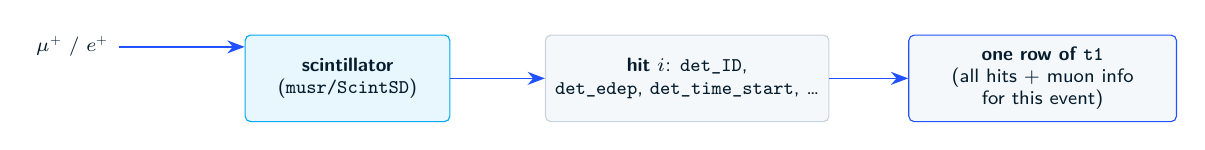
\begin{tikzpicture}[node distance=6mm and 10mm]
  \node[hot,minimum width=26mm] (sc) {\textbf{scintillator}\\(\texttt{musr/ScintSD})};
  \node[box,right=12mm of sc,minimum width=36mm] (h) {\textbf{hit \(i\)}: \texttt{det\_ID},\\\texttt{det\_edep}, \texttt{det\_time\_start}, \dots};
  \node[box,right=of h,minimum width=34mm,draw=eblue] (row) {\textbf{one row of \texttt{t1}}\\(all hits + muon info\\for this event)};
  \draw[arr] ([xshift=-16mm,yshift=4mm]sc.west) node[left,font=\sffamily\scriptsize,text=navy]{\(\mu^+\) / \(e^+\)} -- ([yshift=4mm]sc.west);
  \draw[arr] (sc)--(h); \draw[arr] (h)--(row);
\end{tikzpicture}
\end{center}

\section{The shape of tree \texttt{t1}}
The branches fall into two groups. \emph{Event-level scalars} carry one value per event; \emph{hit arrays} carry \code{det_n} values per event. The most useful of each:

{\tablestyle
\begin{tabularx}{\textwidth}{@{}>{\raggedright\arraybackslash}p{0.36\textwidth} L@{}}
\toprule
\multicolumn{2}{@{}l}{\textbf{Event-level scalars (one per event)}}\\
\midrule
\code{runID}, \code{eventID} & Run and event identifiers.\\
\code{weight} & Event weight (for re-weighted studies).\\
\code{muIniPosX/Y/Z}, \code{muIniMomX/Y/Z} & Initial muon position (mm) and momentum (MeV/c).\\
\code{muIniPolX/Y/Z} & Initial muon polarisation (spin).\\
\code{muDecayDetID} & volumeID of the volume the muon decayed in (\(-1\) for the world).\\
\code{muDecayTime} & Decay time in \si{\micro s} --- the muon-lifetime clock.\\
\code{muDecayPosX/Y/Z}, \code{muDecayPolX/Y/Z} & Position and spin at the moment of decay.\\
\code{muTargetTime}, \code{muTargetPolX/Y/Z} & Muon time and spin on entering a \code{Target} volume (only if one exists).\\
\code{muM0Time}, \code{muM0PolX/Y/Z} & Same, on entering an \code{M0} counter (also \code{M1}, \code{M2}).\\
\code{posIniMomX/Y/Z} & Initial momentum of the decay positron.\\
\midrule
\multicolumn{2}{@{}l}{\textbf{Hit arrays (length \code{det_n})}}\\
\midrule
\code{det_n} & Number of hits in this event.\\
\code{det_ID[]} & Which detector each hit is in (your volumeID).\\
\code{det_edep[]} & Energy deposited in each hit (MeV).\\
\code{det_edep_el/pos/gam/mup/mun[]} & That energy split by \(e^-\), \(e^+\), \(\gamma\), \(\mu^+\), \(\mu^-\).\\
\code{det_time_start[]}, \code{det_time_end[]} & Start and end time of each hit (\si{\micro s}).\\
\code{det_x/y/z[]} & Position of the first step of each hit (mm).\\
\code{det_Vrtx...[]} & Provenance of the depositing particle: vertex position, volume, process, track and particle ID.\\
\bottomrule
\end{tabularx}}

\begin{keypoint}
With default settings the tree has about 80 branches; naming a volume \code{Target}, adding \code{save} planes or enabling optical photons adds whole families (\code{muTarget...}, \code{save_...}, \code{odet_...}), up to a few hundred. You do not need most of them. For a typical positron-counter analysis four branches carry the physics: \code{det_n}, \code{det_ID}, \code{det_edep} and \code{det_time_start}, plus \code{muDecayTime} for lifetimes. Appendix~\ref{app:branches} lists them all.
\end{keypoint}

\begin{pitfall}
A value of \(-1000\) (sometimes \(-999\)) is \musrSim's ``not defined for this event'' marker, not a measurement: \code{muTargetTime} is \(-1000\) when the muon never reached the sample, and the muon branches stay \(-1000\) when the primary is not a muon. Always cut these sentinel values before histogramming or fitting.
\end{pitfall}

\section{Selecting a detector with \texttt{det\_ID}}
Because every counter writes into the same \code{det_edep} array, you isolate one counter by selecting on its \code{det_ID}. This single idiom underlies nearly all \musrSim\ analysis. In a ROOT session on the output of \code{201.mac}:

\begin{lstlisting}[style=cpp,caption={Per-detector spectra in ROOT, selected by \texttt{det\_ID}}]
root -l data/musrSim_jp201.root
root [0] t1->Draw("det_edep", "det_ID==1")                // backward counter B1
root [1] t1->Draw("det_edep", "det_ID==11")               // forward counter F1
root [2] t1->Draw("muDecayTime", "muDecayDetID==201")     // muons that died in the target
root [3] t1->Scan("det_ID:det_edep:det_time_start", "", "colsize=12")
\end{lstlisting}

The second argument to \code{Draw} is a selection evaluated \emph{per hit}, so \code{"det_ID==11"} keeps only hits in the counter you labelled~11.

\section{Controlling the output}
Two kinds of control matter: which events are saved, and which branches are written.

\textbf{Which events.} By default only events with at least one detector hit are kept, since empty events cannot contribute to a real measurement. You can change this:

\begin{lstlisting}[style=mac,caption={Event-selection switches (pick what you need)}]
# default true: keep only events with a hit in any detector
/musr/command storeOnlyEventsWithHits true
# keep only events with a hit in detector 11
/musr/command storeOnlyEventsWithHitInDetID 11
# keep only events whose muon decayed in volume 201
/musr/command storeOnlyEventsWithMuonsDecayedInDetID 201
\end{lstlisting}

(\code{storeOnlyTheFirstTimeHit true} also exists; it stops each track at its first hit and is meant for special studies only.)

\textbf{Which branches.} Trim the tree by switching branches off; \code{201.mac} does this for the optical and vertex families it does not need. A few branches are off by default and must be switched \emph{on}:

\begin{lstlisting}[style=mac,caption={Pruning unused branches keeps files small and fast}]
/musr/command rootOutput odet_ID off
/musr/command rootOutput det_VvvKine off
# off by default -- switch on if needed (fills BxIntegral)
/musr/command rootOutput fieldIntegralBx on
\end{lstlisting}

\begin{checkbuild}
The switch name is usually the branch name, but not always: \code{det_start}/\code{det_end} control \code{det_time_start}/\code{det_time_end}, and \code{fieldIntegralBx} fills \code{BxIntegral}. Only the field integrals, \code{phot_time}, \code{odet_timeC1} and \code{odet_timeCFDarray} accept \code{on}. When unsure, search \code{musrDetectorConstruction.cc} for \code{"rootOutput"}.
\end{checkbuild}

\textbf{Naming the file.} The output path is \code{<dir>/musrSim_jp<NNN>[_<name>].root}. \code{<NNN>} is the leading integer of the macro's file name, zero-padded to three digits; \code{<name>} comes from the second command-line argument or, if none is given, from \code{SetOutputFileName}; \code{<dir>} is \code{data} unless you change it.

\begin{lstlisting}[style=mac,caption={Naming the ROOT file from inside the macro}]
# -> data/musrSim_jp<NNN>.root
/musr/command SetOutputFileName DEFAULT
# or give a suffix: -> data/musrSim_jp<NNN>_myRun.root
# /musr/command SetOutputFileName myRun
# write somewhere other than data/ (the directory must exist)
# /musr/command rootOutputDirectoryName /scratch/me/sims
\end{lstlisting}

\begin{tip}
Prune first, simulate second. Deciding which branches you need before a million-event run can shrink the output several-fold and speed up both writing and later reading. You can always switch a branch back on and re-run a small job to check it.
\end{tip}

\begin{recap}
\begin{itemize}
  \item One stored event \(\rightarrow\) one entry in tree \code{t1}; hits are parallel arrays of length \code{det_n}, split in time by \code{signalSeparationTime}.
  \item Event-level scalars (\code{muDecayTime}, \code{muIniPol...}) versus per-hit arrays (\code{det_edep[]}).
  \item Isolate a counter by selecting on \code{det_ID}; cut the \(-1000\) sentinels.
  \item \code{storeOnly...} chooses which events are kept; \code{rootOutput <branch> off} prunes the tree.
\end{itemize}
\end{recap}
\nextchap{analysing the tree in Python}

\chapter{Analysing the tree in Python}
\label{ch:python}

\begin{willdo}
\begin{itemize}
  \item Open a \musrSim\ ROOT file in Python with \code{uproot} --- no ROOT installation required.
  \item Handle the per-hit jagged arrays correctly with \code{awkward}.
  \item Plot an energy spectrum and fit the muon lifetime.
  \item Package the boilerplate into a small, reusable loader.
\end{itemize}
\end{willdo}

You can analyse \musrSim\ output entirely in Python. The \code{uproot} library reads ROOT files without a ROOT installation, and \code{awkward} gives you fast, NumPy-like operations on the variable-length hit arrays. This chapter builds a complete analysis of the \code{first_sim.mac} output in small pieces. The finished scripts live in \code{doc/scripts/}.

\section{Opening the file}
Install the toolkit once (Section~\ref{sec:conda}), then open the tree by name.

\begin{lstlisting}[style=py,caption={Reading tree \texttt{t1} into arrays}]
import uproot
import awkward as ak
import numpy as np

t = uproot.open("data/musrSim_jp000.root")["t1"]    # the tree is always called t1
print(t.num_entries, "events,", len(t.keys()), "branches")

# Per-hit branches come back as jagged awkward arrays,
# event-level branches as flat arrays.
data = t.arrays(["det_n", "det_ID", "det_edep", "det_time_start",
                 "muDecayTime", "muDecayDetID"], library="ak")
\end{lstlisting}

For the reference run this prints \code{19991 events, 80 branches}.

\begin{keypoint}
\code{det_edep} is \emph{jagged}: event 0 might have two hits and event 1 one. You cannot treat it as a flat column until you either flatten it or select one hit per event. Reaching for \code{np.array(det_edep)} on a jagged branch is the first mistake most people make --- use \code{awkward} instead.
\end{keypoint}

\section{Energy spectra: flattening and masking}
To histogram the energy of every hit, flatten the jagged array. To histogram one counter, mask on \code{det_ID} \emph{before} flattening, so the mask and the data stay aligned.

\begin{lstlisting}[style=py,caption={All-hit spectrum, and a single-counter spectrum}]
import matplotlib.pyplot as plt

all_edep  = ak.flatten(data.det_edep)              # 1-D array of all hits
mask      = data.det_ID == 1                        # jagged boolean, same shape as det_edep
edep_slab = ak.flatten(data.det_edep[mask])         # mask, THEN flatten

fig, ax = plt.subplots(figsize=(6, 4))
ax.hist(np.asarray(all_edep),  bins=100, range=(0, 15), histtype="step", label="all hits")
ax.hist(np.asarray(edep_slab), bins=100, range=(0, 15), histtype="step", label="det_ID == 1")
ax.set_xlabel("Energy deposit [MeV]"); ax.set_ylabel("Hits / bin"); ax.legend()
fig.savefig("edep_spectrum.png", dpi=150)
\end{lstlisting}

\begin{pitfall}
Order matters: \code{ak.flatten(det_edep)[mask]} is wrong, because once \code{det_edep} is flattened the per-event mask no longer lines up with it. Always apply the jagged mask first (\code{det_edep[mask]}) and flatten the result.
\end{pitfall}

To separate the prompt muon hits from the delayed positron hits of Figure~\ref{fig:edep}, mask on time in exactly the same way: \code{data.det_edep[data.det_time_start < 0.01]} keeps hits that started within \SI{10}{ns}.

\section{The muon lifetime}
\code{muDecayTime} is an event-level scalar (in \si{\micro s}), so no flattening is needed --- but you must cut the sentinel for muons without a recorded decay, and you will usually select muons that stopped in a particular volume.

\begin{lstlisting}[style=py,caption={Histogram and fit the muon decay time}]
from scipy.optimize import curve_fit

t_us = np.asarray(data.muDecayTime)
good = np.asarray((data.muDecayDetID == 1) & (data.muDecayTime > 0))   # stopped in the slab
t_us = t_us[good]

counts, edges = np.histogram(t_us, bins=100, range=(0, 15))
centres = 0.5 * (edges[:-1] + edges[1:])

def decay(t, N0, tau, bkg):
    return N0 * np.exp(-t / tau) + bkg

popt, pcov = curve_fit(decay, centres, counts, p0=[counts.max(), 2.2, 1.0],
                       sigma=np.sqrt(counts + 1), absolute_sigma=True)
tau, dtau = popt[1], np.sqrt(pcov[1, 1])
print(f"tau = {tau:.4f} +/- {dtau:.4f} us   (PDG: 2.1970 us)")
\end{lstlisting}

On the 19\,990 muons of the reference run this gives \(\tau = \SI{2.214(20)}{\micro s}\), within one standard deviation of the PDG value (Figure~\ref{fig:lifetime}).

\begin{figure}[h]
\centering
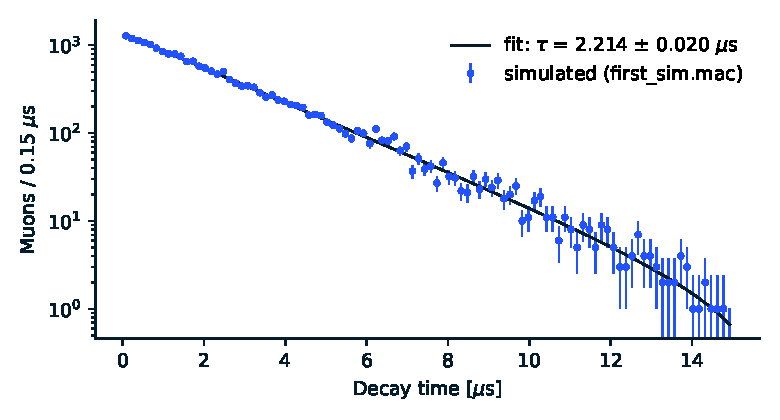
\includegraphics[width=0.78\textwidth]{figures/lifetime.pdf}
\caption{Decay-time distribution of the muons stopped in the slab in \texttt{first\_sim.mac}, with the exponential-plus-constant fit.}
\label{fig:lifetime}
\end{figure}

\begin{physics}
A pure positive-muon sample recovers the free mean life, \(\tau_{\mu^+}\approx\SI{2.197}{\micro s}\). Fit a negative-muon run (\code{/gun/primaryparticle mu-}, with \code{G4MuonMinusCapture} in the physics block) and you will measure something shorter: a \(\mu^-\) stopped in matter can be captured by a nucleus, so its disappearance rate is the sum of decay and capture, and the shift depends strongly on \(Z\) of the stopping material. Seeing that shift emerge from your own simulation is a satisfying check that the physics list is doing its job.
\end{physics}

The complete version of this analysis, which also produces both plots, is \code{doc/scripts/first_analysis.py}; run it from \code{build/run} as \code{python ../../doc/scripts/first_analysis.py}.

\section{A reusable loader}
Wrap the boilerplate once so every later analysis starts from a clean function.

\lstinputlisting[style=py,caption={\texttt{doc/scripts/load.py} --- a small, reusable entry point}]{scripts/load.py}

\begin{tip}
For a whole run directory, \code{uproot.concatenate("data/musrSim_jp201_job*.root:t1", branches, library="ak")} reads and stitches many files at once --- the natural next step when you split a big job across a batch farm (Section~\ref{sec:scale}).
\end{tip}

\begin{recap}
\begin{itemize}
  \item \code{uproot} opens \code{t1} with no ROOT install; per-hit branches are jagged \code{awkward} arrays.
  \item Mask on \code{det_ID} (or time) before flattening; flatten only when you want a 1-D histogram.
  \item \code{muDecayTime} fits to \(\approx\SI{2.197}{\micro s}\) for \(\mu^+\); cut the sentinels first.
  \item A tiny \code{load()} / \code{counter()} pair removes the boilerplate from every future script.
\end{itemize}
\end{recap}
\nextchap{fields, the physics list, and running at scale}

\chapter{Fields, physics, and running at scale}
\label{ch:fields}

\begin{willdo}
\begin{itemize}
  \item Add magnetic and electric fields --- uniform, mapped from a file, and quadrupole.
  \item Understand exactly which physics your run contains, and how to change it.
  \item Enable optical-photon tracking, and know what it costs.
  \item Split a large simulation across many jobs with statistically independent random numbers.
\end{itemize}
\end{willdo}

This chapter collects the capabilities you reach for once the basics work: fields (essential for real \muSR), the physics list, optical photons, and the mechanics of large production runs.

\section{Magnetic and electric fields}
Fields are added with the \code{globalfield} command family and attached to a logical volume. Fields from several elements may overlap; \musrSim\ sums them.

\textbf{Uniform field.} Give the half-dimensions of the box the field fills, the keyword \code{uniform}, the box centre, the host logical volume, then \emph{six} numbers: \(B_x\,B_y\,B_z\) in tesla and \(E_x\,E_y\,E_z\) in kV/mm.

\begin{lstlisting}[style=mac,caption={A uniform \SI{10}{mT} field along $x$, over a \SI{800}{mm} cube at the origin}]
# globalfield <name> <halfX halfY halfZ> uniform <x y z> <logVol> <Bx By Bz> <Ex Ey Ez>
/musr/command globalfield TF 400 400 400 uniform 0 0 0 log_World 0.01 0 0 0 0 0
\end{lstlisting}

\begin{pitfall}
Always give all six field components, even when \(E=0\). The parser reads exactly six numbers; leaving the electric part off leaves those values undefined.
\end{pitfall}

\textbf{Field map.} A mapped field reads a table from a file and scales it, as the GPD solenoid does in \code{201.mac}. The first three numbers are the map's centre; then \code{fromfile}, the table format, the file, the host volume and the field value in tesla:

\begin{lstlisting}[style=mac,caption={A solenoid field from a 2-D field map (from \texttt{201.mac})}]
# globalfield <name> <x y z> fromfile <format> <tablefile> <logVol> <value[T]> [<final> <nSteps>]
/musr/command globalfield centralSolenoidField 0. 0. 0. fromfile 2D GPD_coil_primitive.table log_target 0.03
\end{lstlisting}

The format names the table layout: \code{2D} or \code{3D} (OPERA-style tables), \code{2DB}/\code{2DE} and \code{3DB}/\code{3DE} (magnetic/electric maps in the PSI format), plus a few specialised variants listed in \code{musrTabulatedElementField.cc}. Supplying the two optional trailing numbers --- a final value and a number of steps --- ramps the field linearly with event number, a compact way to simulate a field scan in a single run.

\textbf{Quadrupole.} \code{globalfield <name> <x y z> quadrupole <halfLength> <radius> <fringeFactor> <logVol> <gradient[T/m]>} builds a magnetic quadrupole with fringe fields.

Check what you built, and tune the integration accuracy if needed:

\begin{lstlisting}[style=mac,caption={Verifying the field and tuning the stepping accuracy}]
/musr/command globalfield printFieldValueAtPoint 0 0 0
/musr/command globalfield printparameters
/musr/command globalfield setparameter SetLargestAcceptableStep 200
/musr/command globalfield setparameter SetMinimumEpsilonStep 5e-5
/musr/command globalfield setparameter SetMaximumEpsilonStep 0.001
/musr/command globalfield setparameter SetDeltaOneStep 0.1
\end{lstlisting}

\code{printFieldValueAtPoint} prints, just before the first event, a line such as\\
\code{Field at (0.00, 0.00, 0.00) mm is:  B = (0.01, 0, 0) T,  E = (0, 0, 0) kV/mm}.

\begin{checkbuild}
Always print the field at a few points after defining a mapped field. A map with the wrong axis convention, units or centre offset is the most common silent error in field work, and the printout catches it in seconds. Note also that Geant4~11 refuses a maximum epsilon step above 0.01; \musrSim\ now lowers larger values to 0.01 and tells you so.
\end{checkbuild}

\begin{keypoint}
In a field, \musrSim\ transports the muon spin along with its trajectory --- and keeps precessing it after the muon stops. The recorded \code{muDecayPol...} reflects all the precession the muon underwent, so a transverse field produces the oscillating asymmetry you will build in Chapter~\ref{ch:capstone}.
\end{keypoint}

\section{The physics list, exactly}
\label{sec:physics}
\musrSim\ always uses its own physics list, \code{musrPhysicsList}. Most of it is assembled from your macro (Section~\ref{sec:physicsblock}); a few pieces are fixed in C++:

{\tablestyle
\begin{tabularx}{\textwidth}{@{}>{\raggedright\arraybackslash}p{0.3\textwidth} L@{}}
\toprule
\textbf{Always present} & \textbf{From your macro (\code{/musr/command process ...})}\\
\midrule
Transportation; muon decay \emph{with spin} (\code{G4DecayWithSpin}) for \(\mu^\pm\); multiple scattering and ionisation for other charged hadrons and ions; muonium (\code{Mu}) scattering and decay; radioactive decay for ions when GPS is used. &
\textbf{addProcess} (particle, process, three ordering numbers): \code{G4eMultipleScattering}, \code{G4eIonisation}, \code{G4eBremsstrahlung}, \code{G4eplusAnnihilation}, \code{G4MuMultipleScattering}, \code{G4MuIonisation}, \code{G4MuBremsstrahlung}, \code{G4MuPairProduction}, \code{musrMuFormation}, \code{musrMuEnergyLossLandau}, \code{G4MuonMinusCapture}, \code{G4Scintillation}, \code{G4Cerenkov}, \code{G4StepLimiter}, \code{G4UserSpecialCuts}.\newline
\textbf{addDiscreteProcess}: \code{G4PhotoElectricEffect}, \code{G4ComptonScattering}, \code{G4GammaConversion}, \code{G4GammaConversionToMuons}, \code{G4RayleighScattering}, \code{G4CoulombScattering}, \code{G4OpAbsorption}, \code{G4OpRayleigh}, \code{G4OpBoundaryProcess}, \code{G4OpWLS}.\\
\bottomrule
\end{tabularx}}

Production cuts default to \SI{0.1}{mm} for photons and electrons and can be changed with \code{/musr/command process cutForGamma <mm>} and \code{cutForElectron <mm>}.

Two consequences follow. First, \emph{there is no hadronic physics} for nucleons and pions beyond ionisation and scattering, and no photo- or electro-nuclear reactions: \musrSim\ is an electromagnetic-plus-muon toolkit. If neutron or pion interactions matter to you, that is a C++ change. Second, every example macro's \code{process} block is meaningful: it is your physics.

\begin{pitfall}
An unknown process name stops the run with \code{not implemented in musrPhysicsList.cc}. Older macros sometimes name processes that were never wired in; add the one line to \code{musrPhysicsList::ConstructEM()} --- this edition added \code{G4GammaConversionToMuons} exactly that way --- or remove the line. (\code{/musr/command G4EmExtraPhysics} is still accepted for compatibility, but does nothing.)
\end{pitfall}

For \(\mu^+\) stopping in matter, muonium formation can be modelled with \code{musrMuFormation}; for \(\mu^-\), add \code{G4MuonMinusCapture} as an at-rest process:

\begin{lstlisting}[style=mac,caption={Negative-muon capture at rest}]
/musr/command process addProcess mu- G4MuonMinusCapture 0 -1 -1
\end{lstlisting}

\section{Optical photons}
\label{sec:optical}
For studies of light yield and photodetector timing you can track individual scintillation and Cherenkov photons. It is off by default because it is expensive. Turning it on takes four ingredients, all in the macro; \code{run/110.mac} is a complete working example.

\begin{enumerate}
  \item \code{/musr/command G4OpticalPhotons true}.
  \item Optical properties for each material photons travel in --- a named \code{materialPropertiesTable}, attached with \code{setMaterialPropertiesTable}: refractive index, absorption length, emission spectrum, yield, time constants.
  \item The optical processes: \code{G4Scintillation} (and/or \code{G4Cerenkov}) for the charged particles, and \code{G4OpAbsorption}, \code{G4OpRayleigh}, \code{G4OpBoundaryProcess} for \code{opticalphoton}.
  \item Optical surfaces (\code{opticalSurface}) with an \code{EFFICIENCY} where photons are detected, e.g. a scintillator--APD boundary.
\end{enumerate}

\begin{lstlisting}[style=mac,caption={Optical properties of a plastic scintillator (shortened from \texttt{110.mac}; photon energies in MeV)}]
/musr/command G4OpticalPhotons true
/musr/command materialPropertiesTable optScintMPT RINDEX 2  2.695e-6 3.64618e-6  1.58 1.58
/musr/command materialPropertiesTable optScintMPT SCINTILLATIONYIELD 0 9167.
/musr/command materialPropertiesTable optScintMPT FASTTIMECONSTANT   0 1.32
/musr/command materialPropertiesTable optScintMPT YIELDRATIO         0 1.0
/musr/command setMaterialPropertiesTable optScintMPT G4_PLASTIC_SC_VINYLTOLUENE
/musr/command process addProcess e- G4Scintillation 4 -1 4
/musr/command process addDiscreteProcess opticalphoton G4OpAbsorption
/musr/command process addDiscreteProcess opticalphoton G4OpBoundaryProcess
\end{lstlisting}

When active, the \code{odet_...} branches record photon counts and arrival times per optical detector, and the \code{OPSA} command family simulates the photodetector signal.

\begin{checkbuild}
Geant4~11 renamed the two-component scintillation properties (\code{FASTCOMPONENT} \(\rightarrow\) \code{SCINTILLATIONCOMPONENT1}, \code{FASTTIMECONSTANT} \(\rightarrow\) \code{SCINTILLATIONTIMECONSTANT1}, \code{YIELDRATIO} \(\rightarrow\) \code{SCINTILLATIONYIELD1/2}, and the \code{SLOW...} equivalents). \musrSim\ translates the old names automatically, so both spellings work in your macro.
\end{checkbuild}

\begin{pitfall}
Optical photons can multiply the number of tracked particles per event by thousands, slowing a run by one to two orders of magnitude. Turn them on only for the detector study that needs them, keep the event count modest, and leave them off for geometry, beam and asymmetry work.
\end{pitfall}

\section{Running at scale}
\label{sec:scale}
Physics runs need millions of events, which means many jobs. Each job must use \emph{different random numbers} and write a \emph{differently named} file. The second is easy --- the second command-line argument sets the file suffix. The first needs care.

\begin{keypoint}
How the random engine is seeded is set by \code{/musr/run/randomOption}:
\begin{itemize}
  \item \code{0} (default) --- no seeding: every run of the same macro produces the \emph{same} events;
  \item \code{1} --- seed from the clock \emph{plus} 100 \(\times\) the seed offset (third command-line argument or \code{SetRndSeedOffset});
  \item \code{2} --- re-seed each event with its event number: perfectly reproducible, event by event, and therefore \emph{identical} across jobs;
  \item \code{5} --- a fixed seed from \code{/musr/command SetRndSeed <n>} (fully reproducible run).
\end{itemize}
For independent parallel jobs use \textbf{option 1} with a different offset per job.
\end{keypoint}

We tested this directly: two 300-event jobs of \code{first_sim.mac} with seed offsets 1 and 2 produced \emph{identical} muon decay times under options 0 and 2, and different ones under option 1.

\begin{lstlisting}[style=mac,caption={Settings for production jobs}]
/musr/run/randomOption 1
/musr/run/howOftenToPrintEvent 10000
# wall-clock guard in seconds: stop the run cleanly before the batch limit
/musr/command maximumRunTimeAllowed 82800
\end{lstlisting}

\begin{lstlisting}[style=sh,caption={A simple job split, then merge with ROOT's \texttt{hadd}}]
for i in $(seq 1 50); do
  ../musrSim 201.mac job${i} ${i} > log_job${i}.txt 2>&1 &
done
wait
# outputs: data/musrSim_jp201_job1.root ... data/musrSim_jp201_job50.root
hadd data/musrSim_jp201_merged.root data/musrSim_jp201_job*.root
\end{lstlisting}

On an HTCondor farm the same idea becomes a submit file with \code{Queue 50}, passing \code{$(Process)} as both the name suffix and the seed offset.

\begin{pitfall}
Option~1 seeds from the clock, so a job is not reproducible after the fact unless you note its seeds: they are printed at the start of the log (\code{seed1: ...; seed2: ...}). Keep the logs. If you need bit-exact reproducibility of a single job, use option~5 with an explicit \code{SetRndSeed} per job instead.
\end{pitfall}

\begin{tip}
Two run-time safety valves. \code{maximumRunTimeAllowed} defaults to \SI{85000}{s} (about 23.6 hours): a longer job stops itself there, writing what it has --- raise it for multi-day runs. And to stop a running job gracefully, create a file named after its macro with \code{.stop} instead of \code{.mac} (\code{touch 201.stop}): the run ends after the current event and the ROOT file is written normally.
\end{tip}

\begin{tip}
Merge with \code{hadd} when you want a single ROOT file; for Python analysis you can skip the merge: \code{uproot.concatenate("data/musrSim_jp201_job*.root:t1", ...)} reads the whole set directly.
\end{tip}

\begin{recap}
\begin{itemize}
  \item \code{globalfield ... uniform} needs six field numbers; \code{... fromfile <format>} reads a map; always \code{printFieldValueAtPoint}.
  \item \code{musrPhysicsList} is the only physics list; your \code{process} lines are your EM physics; there is no hadronic physics.
  \item \code{G4OpticalPhotons true} plus material tables, processes and surfaces enables photon tracking --- at a large speed cost.
  \item Parallel jobs need \code{randomOption 1} and a different seed offset each; merge with \code{hadd} or read all files in \code{uproot}.
\end{itemize}
\end{recap}
\nextchap{a complete \muSR\ asymmetry measurement}

\chapter{Capstone: a transverse-field asymmetry measurement}
\label{ch:capstone}

\begin{willdo}
\begin{itemize}
  \item Assemble geometry, field, physics, beam and output into one simulation.
  \item Reproduce muon-spin precession in a transverse magnetic field.
  \item Build the asymmetry signal and fit a precession frequency.
  \item Recover the field you set from the frequency you measured.
\end{itemize}
\end{willdo}

Everything so far has been groundwork. Here we run a complete, if idealised, transverse-field muon spin rotation experiment: muons stop in a sample sitting in a magnetic field perpendicular to their spin, their spins precess, and the decay positrons are counted in two opposing detectors. The normalised difference of those counts oscillates at the Larmor frequency --- and from it we recover the field.

\section{The physics in one paragraph}
A muon spin in a magnetic field \(B\) precesses at the Larmor frequency \(f=(\gamma_\mu/2\pi)\,B\), with \(\gamma_\mu/2\pi\approx\SI{135.54}{MHz/T}\). The decay positron is emitted preferentially along the muon spin at the instant of decay. If the spin starts along the beam axis (\(z\)) and the field points along \(x\), the spin rotates in the \(y\)--\(z\) plane, so its \(y\)-component swings as \(\sin(2\pi f t)\). Two counters facing each other along \(\pm y\) therefore see their positron rates rise and fall in antiphase. The asymmetry
\[
A(t)=\frac{N_\mathrm{D}(t)-N_\mathrm{U}(t)}{N_\mathrm{D}(t)+N_\mathrm{U}(t)}
\]
cancels the exponential decay common to both counters and leaves a clean oscillation.

\begin{center}
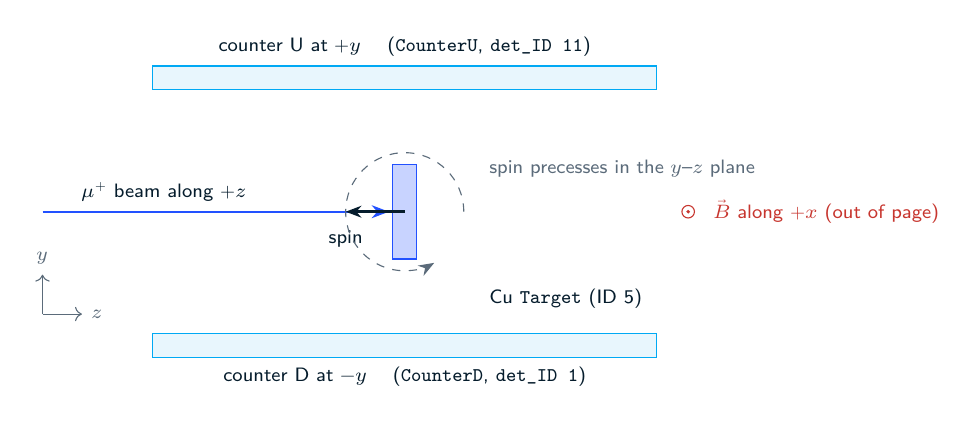
\begin{tikzpicture}[font=\sffamily\scriptsize]
  \fill[cyanbg] (-3.2,1.55) rectangle (3.2,1.85);
  \draw[cyan] (-3.2,1.55) rectangle (3.2,1.85);
  \node[text=navy,above] at (0,1.85) {counter U at \(+y\) \quad (\texttt{CounterU}, \texttt{det\_ID 11})};
  \fill[cyanbg] (-3.2,-1.85) rectangle (3.2,-1.55);
  \draw[cyan] (-3.2,-1.85) rectangle (3.2,-1.55);
  \node[text=navy,below] at (0,-1.85) {counter D at \(-y\) \quad (\texttt{CounterD}, \texttt{det\_ID 1})};
  \fill[eblue!25] (-0.15,-0.6) rectangle (0.15,0.6);
  \draw[eblue] (-0.15,-0.6) rectangle (0.15,0.6);
  \node[text=navy,anchor=west] at (0.95,-1.1) {Cu \texttt{Target} (ID 5)};
  \draw[arr] (-4.6,0) -- (-0.2,0) node[pos=0.35,above,text=navy]{\(\mu^+\) beam along \(+z\)};
  \draw[-{Stealth[length=2mm]},navy,line width=0.9pt] (0,0) -- (-0.75,0) node[pos=1,below=3pt,text=navy]{spin};
  \draw[-{Stealth[length=2mm]},muted,dashed] (0.75,0) arc (0:300:0.75 and 0.75);
  \node[text=muted,anchor=west] at (0.95,0.55) {spin precesses in the \(y\)--\(z\) plane};
  \node[circle,draw=pitred,inner sep=1.6pt] (b) at (3.6,0) {}; \fill[pitred] (b) circle (0.7pt);
  \node[text=pitred,anchor=west] at (3.8,0) {\(\vec B\) along \(+x\) (out of page)};
  \draw[->,muted] (-4.6,-1.3) -- (-4.1,-1.3) node[right]{\(z\)};
  \draw[->,muted] (-4.6,-1.3) -- (-4.6,-0.8) node[above]{\(y\)};
\end{tikzpicture}
\end{center}

\section{The macro}
The geometry is a copper sample named \code{Target} and two scintillator plates, plus a uniform transverse field over the whole world and the standard physics block. The sample's name switches on the \code{muTarget...} branches, and the run keeps only muons that decayed inside it. The macro ships as \code{run/tf_musr.mac}:

\lstinputlisting[style=mac,caption={\texttt{tf\_musr.mac} --- a complete transverse-field experiment},label=lst:tf]{../run/tf_musr.mac}

\begin{lstlisting}[style=sh,caption={Run it (about 1.5 minutes on one core)}]
cd build/run
mkdir -p data
../musrSim tf_musr.mac        # -> data/musrSim_jp000_tf.root (suffix from SetOutputFileName)
\end{lstlisting}

The log confirms the field just before the first event: \code{Field at (0.00, 0.00, 0.00) mm is: B = (0.01, 0, 0) T}.

\begin{physics}
Surface muons at \SI{29.8}{MeV/c} stop within a fraction of a millimetre, so nearly all of them come to rest inside the \SI{6}{mm}-thick copper sample and decay there. The line \code{storeOnlyEventsWithMuonsDecayedInDetID 5} discards the few that stop elsewhere, so the analysis sees a clean sample-stopped population regardless of the exact stopping profile. Copper is also a good choice physically: muons in a non-magnetic metal do not form muonium and keep their full polarisation.
\end{physics}

\section{The analysis}
Load the tree, keep sample-stopped muons, and split the decay times by which counter caught the positron. Events in which \emph{both} counters fired are ambiguous and dropped. The exponential lifetime divides out of the asymmetry, leaving the precession.

\lstinputlisting[style=py,caption={\texttt{doc/scripts/asymmetry.py} --- from ROOT file to Larmor frequency},label=lst:asym]{scripts/asymmetry.py}

\section{What you should see}
In our reference run, 26\,224 positrons were counted in U and 25\,956 in D. The fit gives
\[
f = \SI{1.3530(20)}{MHz}\quad\Rightarrow\quad B = \frac{f}{\gamma_\mu/2\pi} = \SI{9.983(15)}{mT},
\]
within about one standard deviation of the \SI{10.000}{mT} we set --- a full round trip from a number in a macro to a field recovered from simulated positron counts (Figure~\ref{fig:asym}). The amplitude, \(A_0 = 0.266(9)\), sits below the maximum muon-decay asymmetry of \(1/3\) (averaged over all positron energies) because each counter accepts positrons over a wide range of angles.

\begin{figure}[h]
\centering
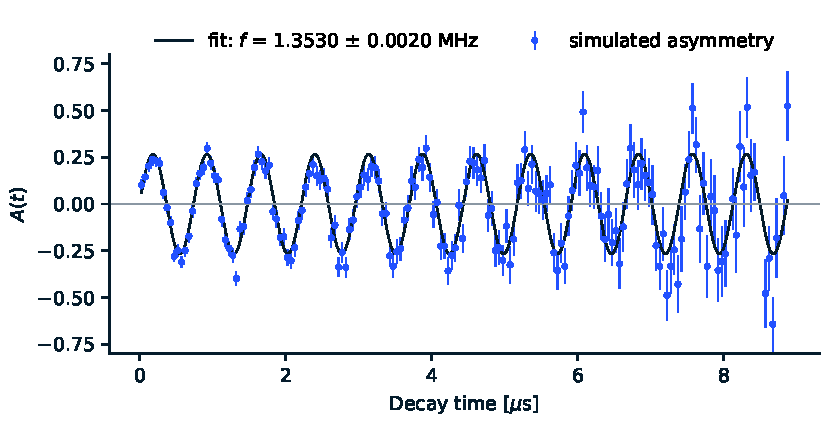
\includegraphics[width=0.86\textwidth]{figures/asymmetry.pdf}
\caption{Simulated positron asymmetry \(A(t)\) from \texttt{tf\_musr.mac} with the damped-sine fit. Error bars grow at late times as the surviving muons run out.}
\label{fig:asym}
\end{figure}

\begin{keypoint}
This closes the loop of the whole book. Geometry (Chapter~\ref{ch:geometry}) placed the counters; the physics block (Chapter~\ref{ch:macro}) let the muons stop and the positrons deposit energy; the field (Chapter~\ref{ch:fields}) drove the precession; the beam and spin (Chapter~\ref{ch:beam}) set the initial condition; the ROOT tree (Chapter~\ref{ch:output}) recorded \code{det_ID} and \code{muDecayTime}; and Python (Chapter~\ref{ch:python}) turned them into a number with a physical meaning.
\end{keypoint}

\begin{tip}
Turn this into a study. Scan the field by editing the one \code{0.01} in the macro, run each value (give each run its own suffix on the command line), and plot fitted frequency against set field --- it should be a straight line of slope \(\gamma_\mu/2\pi\). For a mapped field, the \code{<final> <nSteps>} ramp of Chapter~\ref{ch:fields} scans the field within a single run. Either is a genuine, if small, piece of \muSR\ physics.
\end{tip}

\begin{recap}
\begin{itemize}
  \item A complete experiment is a sample, two counters, a transverse field, the physics block and a polarised beam.
  \item The asymmetry \((N_\mathrm{D}-N_\mathrm{U})/(N_\mathrm{D}+N_\mathrm{U})\) cancels the lifetime and exposes the precession.
  \item Fitting the oscillation recovers the field you set, via \(f=(\gamma_\mu/2\pi)B\): \SI{9.983(15)}{mT} for \SI{10}{mT} set.
  \item Every skill from Chapters~\ref{ch:macro}--\ref{ch:fields} appears here as one part of a single physics result.
\end{itemize}
\end{recap}
\nextchap{troubleshooting, and reading the source}

\chapter{Troubleshooting, and reading the source}
\label{ch:trouble}

\begin{willdo}
\begin{itemize}
  \item Diagnose the common build, run-time and analysis failures quickly.
  \item Turn ``unknown keyword'' into a ten-second source lookup.
  \item Know which source file answers which kind of question.
  \item Build the validation habits that keep simulated numbers trustworthy.
\end{itemize}
\end{willdo}

\musrSim\ is a forked, evolving codebase, so the most valuable long-term skill is not memorising commands but knowing how to interrogate your own copy. This short chapter is a field guide to doing exactly that.

\section{Common failures at a glance}
{\tablestyle
\begin{tabularx}{\textwidth}{@{}>{\raggedright\arraybackslash}p{0.38\textwidth} L@{}}
\toprule
\textbf{Symptom} & \textbf{Most likely cause and fix}\\
\midrule
Build: \code{Could NOT find Geant4} / \code{root-config} missing & Environment not set up. Activate the conda environment, or source \code{geant4.sh} and \code{thisroot.sh}, before \code{cmake}.\\
Build: \code{unsuitable version} of EXPAT or another library & CMake mixed system and conda libraries. Configure with \code{-DCMAKE_PREFIX_PATH=$CONDA_PREFIX}.\\
Run stops: \code{Root output file ... can not be created} & No \code{data/} directory where you launched. \code{mkdir -p data}.\\
Run stops: \code{Unknown keyword requested} & A \code{/musr/command} keyword your build does not implement, or a typo. Look it up (Section~\ref{sec:rejected}).\\
Run stops: \code{not implemented in musrPhysicsList.cc} & A process name the physics list does not know (Section~\ref{sec:physics}).\\
Run stops: \code{Logical Volume "..." not found} & Mother written without \code{log_}, misspelled, or constructed after the daughter.\\
Run stops: \code{Field map file not found} & The map is not in \code{build/run}; put it in \code{run/} and re-run \code{cmake ../}.\\
Tree is empty, or muons never stop & No physics block in the macro (Section~\ref{sec:physicsblock}), or nothing reaches a sensitive volume.\\
Geometry or physics lines ignored & They are in a file pulled in with \code{/control/execute}; \code{/musr/command} lines must be in the main macro (Section~\ref{sec:tworeads}).\\
Overlap reported during construction & A daughter exceeds or intersects its mother, or a half-length is wrong (Chapter~\ref{ch:geometry}).\\
Parallel jobs give identical results & Seeding: use \code{/musr/run/randomOption 1} with a different offset per job (Section~\ref{sec:scale}).\\
Histogram spikes at \(-1000\) & Uncut sentinel values (Chapter~\ref{ch:output}).\\
Fit returns nonsense & Jagged array flattened before masking, or starved bins at late time (Chapter~\ref{ch:python}).\\
\bottomrule
\end{tabularx}}

\section{When a command is rejected}
\label{sec:rejected}
For \code{/musr/command} lines, \musrSim\ prints \code{E R R O R ... Unknown keyword requested} with the offending line and stops. For \code{/gun}, \code{/musr/run} and Geant4 commands, Geant4 reports \code{command not found} and interrupts the batch. Either way the command does not exist in your build --- do not fight it; find out what does exist:

\begin{lstlisting}[style=sh,caption={Confirm a command against your own source}]
# 1. UI commands (/gun, /musr/run, Geant4): ask the running executable
../musrSim first_sim.mac idle      # then: ls /gun/   help /gun/vertexsigma

# 2. /musr/command keywords: grep the parsers
grep -n '"storeOnlyEventsWithHits"' src/musrDetectorConstruction.cc
grep -n '"globalfield"'             src/musrDetectorConstruction.cc
grep -n 'stringProcessName=='       src/musrPhysicsList.cc
\end{lstlisting}

The grep tells you instantly whether the keyword is implemented, and the \code{sscanf} a few lines below the match tells you its exact argument order --- more reliable than any manual, including this one.

\section{A map of the source}
You do not need to read the whole codebase. A handful of files answer almost every question.

{\tablestyle
\begin{tabularx}{\textwidth}{@{}>{\raggedright\arraybackslash}p{0.4\textwidth} L@{}}
\toprule
\textbf{File} & \textbf{Answers questions about}\\
\midrule
\code{musrSim.cc} & Start-up, command-line arguments, run modes, output-name pre-scan, the order of initialisation.\\
\code{src/musrDetectorConstruction.cc} & Every \code{/musr/command} keyword except \code{process}: solids, rotations, materials, \code{globalfield}, \code{rootOutput}, \code{visattributes}, the magic volume names.\\
\code{src/musrPhysicsList.cc} & \code{/musr/command process ...}: which processes exist and how they are added.\\
\code{src/musrRootOutput.cc} & Every ROOT branch: names, types, units and default on/off state; the output file name.\\
\code{src/musrPrimaryGeneratorAction.cc}, \code{...Messenger.cc} & Every \code{/gun/} command: vertex, momentum, spin, TURTLE, GPS switch-over, EcoMug and CRY.\\
\code{src/musrScintSD.cc} & What a hit is and how \code{det_...} values are computed; hit merging and event selection.\\
\code{src/musrSteppingAction.cc}, \code{musrEventAction.cc} & Per-step and per-event logic: \code{kill}/\code{shield} volumes, \code{save} planes, run-time limits, the \code{.stop} file.\\
\code{src/musrDetectorMessenger.cc} & \code{/musr/run/...}: random-number options.\\
\code{src/F04*.cc}, \code{musrTabulatedElementField.cc} & Field elements, field maps and integration accuracy.\\
\code{include/EcoMug.h}, \code{src_cry/} & The cosmic-ray generator libraries.\\
\bottomrule
\end{tabularx}}

\begin{keypoint}
The pattern to internalise: a \code{/musr/command X} line is parsed by a long \code{if/else if (strcmp(...,"X")==0)} chain in \code{musrDetectorConstruction.cc} (or \code{musrPhysicsList.cc} for \code{process}), and a ROOT branch is declared once in \code{musrRootOutput.cc}. Those files, searched with \code{grep}, are the definitive reference for this toolkit.
\end{keypoint}

\section{Validation habits}
Simulated numbers are only as good as your scepticism. Four cheap checks catch most mistakes.
\begin{enumerate}
  \item \textbf{Look at the geometry} before any physics run, and confirm every overlap check says \code{OK}.
  \item \textbf{Run a known case.} A \(\mu^+\) lifetime fit must return \SI{2.197}{\micro s}; a field you set must come back out of a precession fit (Chapter~\ref{ch:capstone}). If a calibration you understand is wrong, stop.
  \item \textbf{Check counts and sentinels.} Compare the number of stored events, the \code{det_n} distribution and the fraction of \(-1000\) values against expectation before trusting a spectrum.
  \item \textbf{Vary one thing.} Change the field, the momentum or the geometry by a known amount and confirm the result moves the way physics says it should.
\end{enumerate}

\begin{recap}
\begin{itemize}
  \item Most failures are environment, a missing \code{data/}, a missing physics block, geometry overlaps, or uncut sentinels.
  \item A rejected command means grep the source or ask the executable --- never guess.
  \item \code{musrDetectorConstruction.cc}, \code{musrPhysicsList.cc} and \code{musrRootOutput.cc} are the real reference.
  \item Validate with a known lifetime and a known field before trusting anything new.
\end{itemize}
\end{recap}
\nextchap{reference appendices}


\appendix
\chapter{Command quick reference}
\label{app:commands}
A summary of every command family, checked against the \texttt{musrSim-upgrade} source (\code{musrDetectorConstruction.cc}, \code{musrPhysicsList.cc}, \code{musrPrimaryGeneratorMessenger.cc}, \code{musrDetectorMessenger.cc}). Units inside \code{/musr/command} lines are fixed: mm, degrees, tesla, kV/mm, ns. \code{/gun} commands take an explicit unit.

\eyebrow{Geometry}
\begin{lstlisting}[style=mac]
/musr/command construct <solid> <name> <dims...> <material> <x y z> <log_mother> <rot> <sens> <volID>
/musr/command construct stl <name> <file.stl> <material> <x y z> <log_mother> <rot> <sens> <volID>
/musr/command rotation <name> <ax ay az angle>        # axis-angle (angle != 0)
/musr/command rotation <name> <phi theta psi>         # Euler angles
/musr/command arrayDef <name> <n> <v1 ... vn>         # arrays for polyconeA/B
/musr/command visattributes <log_name | material> <colour | invisible>
# solids: box tubs cons sphere trd para torus polyconeA polyconeB stl + composites (Appendix C)
# sens:   musr/ScintSD (detector) | dead (inert)
# magic names: World, Target, M0/M1/M2, *save*, kill*, shield*
\end{lstlisting}

\eyebrow{Physics}
\begin{lstlisting}[style=mac]
/musr/command process addProcess <particle> <G4Process> <atRest> <alongStep> <postStep>
/musr/command process addDiscreteProcess <particle> <G4Process>
/musr/command process cutForGamma <mm>        /musr/command process cutForElectron <mm>
/musr/command G4OpticalPhotons <true|false>
/musr/command materialPropertiesTable <table> <PROPERTY> <n> <energies...> <values...>   # n=0: constant
/musr/command setMaterialPropertiesTable <table> <material>
/musr/command opticalSurface <name> <phys_vol1> <phys_vol2> <type> <finish> <model> [<table>]
/musr/command killAllElectrons|killAllPositrons|killAllGammas|killAllNeutrinos <true|false>
/musr/command SetUserLimits <log_name> ...      /musr/command region define <region> <log_name>
\end{lstlisting}

\eyebrow{Fields}
\begin{lstlisting}[style=mac]
/musr/command globalfield <name> <hx hy hz> uniform <x y z> <log_vol> <Bx By Bz> <Ex Ey Ez>
/musr/command globalfield <name> <x y z> fromfile <format> <file> <log_vol> <value> [<final> <nSteps>]
/musr/command globalfield <name> <x y z> quadrupole <halfLength> <radius> <fringe> <log_vol> <gradient>
/musr/command globalfield setparameter <SetLargestAcceptableStep|SetMinimumEpsilonStep|
              SetMaximumEpsilonStep|SetDeltaOneStep|SetDeltaIntersection|SetMaxLoopCount> <value>
/musr/command globalfield printparameters
/musr/command globalfield printFieldValueAtPoint <x y z>
\end{lstlisting}

\eyebrow{Output and run control}
\begin{lstlisting}[style=mac]
/musr/command SetOutputFileName <DEFAULT | suffix>     # data/musrSim_jp<NNN>[_suffix].root
/musr/command rootOutputDirectoryName <dir>
/musr/command rootOutput <branch-switch> <off | on>
/musr/command storeOnlyEventsWithHits <true|false>
/musr/command storeOnlyEventsWithHitInDetID <id>
/musr/command storeOnlyEventsWithMuonsDecayedInDetID <id>
/musr/command storeOnlyTheFirstTimeHit <true|false>
/musr/command signalSeparationTime <ns>
/musr/command maximumRunTimeAllowed <s>                # default 85000
/musr/command maximumTimePerEvent <s>
/musr/command maximumNrOfStepsPerTrack <n>
/musr/command SetRndSeedOffset <n>     /musr/command SetRndSeed <n>
/musr/run/randomOption <0|1|2|3|4|5>   /musr/run/howOftenToPrintEvent <n>
/musr/run/runID <n>
/run/beamOn <N>
\end{lstlisting}

\eyebrow{Beam (particle gun)}
\begin{lstlisting}[style=mac]
/gun/primaryparticle <mu+|mu-|e+|e-|proton|...>
/gun/vertex <x y z> mm             /gun/vertexsigma <sx sy sz> mm    # +Gaussian, -uniform
/gun/vertexboundary <rMax zMin zMax> mm                /gun/vertexrelativer <rMax> mm
/gun/momentum <p> MeV              /gun/kenergy <T> MeV               /gun/momentumsmearing <sigma> MeV
/gun/momentumboundary <pMin pMax 0> MeV
/gun/direction <dx dy dz>          /gun/tilt <ax ay 0> deg            /gun/tiltsigma <sx sy 0> deg
/gun/pitch <angle> deg
/gun/muonPolarizVector <x y z>     /gun/muonPolarizFraction <-1..1>
/gun/decaytimelimits <min max meanlife> ns                  # active only if max > 0
/gun/starttime <t> ns  /gun/starttimesigma <t> ns  /gun/meanarrivaltime <t> ns
/gun/turtlefilename <file>  /gun/turtleZ0position <z> mm  /gun/turtleMomentumScalingFactor <f>
/gun/turtleInterpretAxes <mode>  /gun/turtleMomentumBite <...>  /gun/turtleFirstEventNr <n>
\end{lstlisting}

\eyebrow{Cosmic rays (Appendix \ref{app:cosmics})}
\begin{lstlisting}[style=mac]
/gun/ecomug/useEcoMug true
/gun/ecomug/shapeConstruct <plane|sphere|cylinder> <s1 s2 cx cy cz>          # mm
/gun/ecomug/constraints <pMin pMax thetaMin thetaMax phiMin phiMax>       # MeV/c, deg
/gun/cry/useCRY true
/gun/cry/input <key value>  ...  then  /gun/cry/update       # or: /gun/cry/file <setup file>
/gun/cosmic_v1 <true|false>
\end{lstlisting}

\chapter{ROOT output branch reference}
\label{app:branches}
The tree is named \code{t1}. Per-hit arrays all have length \code{det_n}. Positions are in mm, times in \si{\micro s}, energies in MeV and momenta in MeV/c unless noted; \(-1000\) marks ``undefined''. Switch off what you do not need with \code{rootOutput <switch> off}; the switch name differs from the branch name where noted.

\eyebrow{Event level (one value per event)}
{\tablestyle
\begin{tabularx}{\textwidth}{@{}>{\raggedright\arraybackslash}p{0.42\textwidth} L@{}}
\toprule
\code{runID}, \code{eventID}, \code{weight} & Identifiers and event weight.\\
\code{timeToNextEvent} & For continuous-beam studies (\code{/gun/meanarrivaltime}).\\
\code{BFieldAtDecay} & \(B_x,B_y,B_z,E_x,E_y,E_z\) at the muon decay point.\\
\code{muIniTime}, \code{muIniPosX/Y/Z} & Muon start time and position.\\
\code{muIniMomX/Y/Z}, \code{muIniPolX/Y/Z} & Muon initial momentum and polarisation.\\
\code{parIniTime}, \code{parIniPosX/Y/Z}, \code{parIniMomX/Y/Z}, \code{parID} & Primary-particle start values (any species; filled by EcoMug and CRY).\\
\code{muDecayDetID}, \code{muDecayTime} & Volume of decay (volumeID) and decay time.\\
\code{muDecayPosX/Y/Z}, \code{muDecayPolX/Y/Z} & Position and spin at decay.\\
\code{muTargetTime}, \code{muTargetPolX/Y/Z}, \code{muTargetMomX/Y/Z} & On entering a \code{Target} volume (only when one exists).\\
\code{muM0Time}, \code{muM0PolX/Y/Z} (also \code{M1}, \code{M2}) & On entering \code{M0}--\code{M2} counters (only when they exist).\\
\code{posIniMomX/Y/Z}, \code{elIniMomX/Y/Z} & Initial momentum of the decay positron / electron.\\
\code{nFieldNomVal}, \code{fieldNomVal} & Nominal values of the defined field elements.\\
\code{BxIntegral}, \code{ByIntegral}, \code{BzIntegral}, \code{BzIntegral1..3} & Field path integrals; off by default (switches \code{fieldIntegralBx}, \dots).\\
\code{nOptPhot}, \code{nOptPhotDet}, \code{phot_time} & Optical-photon counts and times (optical runs only).\\
\bottomrule
\end{tabularx}}

\eyebrow{Detector hits (arrays of length det\_n)}
{\tablestyle
\begin{tabularx}{\textwidth}{@{}>{\raggedright\arraybackslash}p{0.42\textwidth} L@{}}
\toprule
\code{det_n} & Number of hits this event.\\
\code{det_ID} & Detector volumeID of each hit.\\
\code{det_edep} & Total energy deposited per hit.\\
\code{det_edep_el/pos/gam/mup/mun} & Deposit by \(e^-\), \(e^+\), \(\gamma\), \(\mu^+\), \(\mu^-\).\\
\code{det_kine_mup/mun} & Kinetic energy of the \(\mu^\pm\) at its step in the hit.\\
\code{det_time_start}, \code{det_time_end} & Hit start and end time (switches \code{det_start}, \code{det_end}).\\
\code{det_x/y/z}, \code{det_x/y/z_mup}, \code{det_x/y/z_mun} & First-step position of the hit, and of the \(\mu^\pm\) in it.\\
\code{det_nsteps}, \code{det_length}, \code{det_kine} & Step count, path length, kinetic energy of the first particle.\\
\code{det_VrtxKine}, \code{det_VrtxX/Y/Z}, \code{det_VrtxVolID}, \code{det_VrtxProcID}, \code{det_VrtxTrackID}, \code{det_VrtxPrtTrackID}, \code{det_VrtxParticleID} & Provenance of the depositing particle: its creation vertex, volume, process, track, parent track and particle type.\\
\code{det_Vvv...} (same set) & The same provenance traced one step further back, to an ancestor of the depositing particle (see \code{musrScintSD.cc} for the exact rule).\\
\bottomrule
\end{tabularx}}

\eyebrow{Tracking planes and optical detectors (only when used)}
{\tablestyle
\begin{tabularx}{\textwidth}{@{}>{\raggedright\arraybackslash}p{0.42\textwidth} L@{}}
\toprule
\code{save_n}, \code{save_detID}, \code{save_particleID} & Crossings recorded by \code{*save*} volumes.\\
\code{save_ke}, \code{save_time}, \code{save_x/y/z}, \code{save_px/py/pz} & Kinematics at the plane.\\
\code{save_polx/poly/polz} & Spin at the plane.\\
\code{odet_n}, \code{odet_ID}, \code{odet_nPhot}, \code{odet_nPhotPrim} & Per optical detector: photon counts.\\
\code{odet_timeFirst/Second/Third}, \code{odet_timeA..D}, \code{odet_timeMean}, \code{odet_timeLast} & Photon arrival-time estimators.\\
\code{odet_timeCFD}, \code{odet_amplCFD}, \code{odet_timeC1..}, \code{odet_timeCFDarray} & Simulated signal (OPSA): constant-fraction timing and amplitude.\\
\bottomrule
\end{tabularx}}

\chapter{Materials and solids reference}
\label{app:solids}

\eyebrow{Frequently used NIST materials}
{\tablestyle
\begin{tabularx}{\textwidth}{@{}>{\raggedright\arraybackslash}p{0.45\textwidth} L@{}}
\toprule
\code{G4_Galactic} & Ideal vacuum.\\
\code{G4_AIR} & Air (the usual world).\\
\code{G4_PLASTIC_SC_VINYLTOLUENE} & Plastic scintillator.\\
\code{G4_Cu}, \code{G4_Al}, \code{G4_Pb}, \code{G4_Fe}, \code{G4_W}, \code{G4_Ag}, \code{G4_Au} & Common metals.\\
\code{G4_MYLAR}, \code{G4_KAPTON}, \code{G4_POLYETHYLENE} & Films and light materials.\\
\code{G4_WATER}, \code{G4_Si}, \code{G4_Ge}, \code{G4_CONCRETE} & Water, semiconductors, concrete.\\
\bottomrule
\end{tabularx}}

Any name from Geant4's NIST database works (\code{G4_...}). In addition, \code{musrDetectorConstruction::DefineMaterials()} defines: \code{Scintillator}, \code{Mylar}, \code{Brass}, \code{Steel}, \code{Water}, \code{Aerogel}, \code{LaBr3}, \code{Macor}, \code{MCPglass}, \code{MgO}, \code{SiO2}, \code{Al2O3}, \code{K2O}, \code{B2O3}, \code{Air}, \code{Vacuum}, \code{ArgonGas}, \code{Rock}, \code{Concrete}, low-pressure air (\code{Air1mbar}, \code{AirE1mbar} \dots \code{AirE6mbar}) and a series of helium gases (\code{HeliumGas5mbar} \dots \code{HeliumGas100mbar}, \code{HeliumGasSat4K}, \dots).

\eyebrow{Solids and their dimension fields (mm, deg; box/tube extents are half-lengths)}
{\tablestyle
\begin{tabularx}{\textwidth}{@{}l L@{}}
\toprule
\code{box} & half-x, half-y, half-z\\
\code{tubs} & rMin, rMax, half-z, \(\phi_0\), \(\Delta\phi\)\\
\code{cons} & rMin1, rMax1, rMin2, rMax2, half-z, \(\phi_0\), \(\Delta\phi\)\\
\code{sphere} & rMin, rMax, \(\phi_0\), \(\Delta\phi\), \(\theta_0\), \(\Delta\theta\)\\
\code{trd} & half-x1, half-x2, half-y1, half-y2, half-z\\
\code{para} & half-x, half-y, half-z, \(\alpha\), \(\theta\), \(\phi\)\\
\code{torus} & rMin, rMax, rTorus, \(\phi_0\), \(\Delta\phi\)\\
\code{polyconeA} & \(\phi_0\), \(\Delta\phi\), \(n\), arrays z, rInner, rOuter (from \code{arrayDef})\\
\code{polyconeB} & \(\phi_0\), \(\Delta\phi\), \(n\), arrays r, z\\
\code{stl} & an STL file name instead of dimensions (CADMesh import, mm)\\
\bottomrule
\end{tabularx}}

\textbf{Composite shapes} hard-coded in \code{musrDetectorConstruction.cc} (read the source for their parameters): \code{boxbox}, \code{tubsbox}, \code{tubsbox2}, \code{tubsboxsegm}, \code{cylpart}, \code{uprofile}, \code{cruciform}, \code{trd90y}, \code{tubeWithWindows}, \code{TubeWithTubeHole}, \code{TubeWithHolePlusTubeHole}, \code{TubeWithHoleAndTubeHole}, \code{BarWithBevelledEdgesX}, \code{alcSupportPlate}, and the PSI instrument parts \code{GPDcollimator}, \code{GPDmHolder}, \code{GPDsampleHolderA}, \code{GPSforward}, \code{GPSbackward}, \code{GPSbackwardVeto}.

\chapter{An annotated skeleton macro}
\label{app:skeleton}
Copy this template and fill in the bracketed parts. It is ordered for readability --- geometry, physics, output, beam, go --- and keeps every \code{/musr/command} line in the one file you pass on the command line (Section~\ref{sec:tworeads}).

\begin{lstlisting}[style=mac,caption={A reusable starting point for a new simulation}]
# ================================================================
# <name>.mac -- one-line description
# /musr/command units: mm, deg, tesla, kV/mm, ns
# ================================================================

# ---- rotation matrices (define BEFORE the volumes that use them) ----
# 90 deg about y
/musr/command rotation rotA 0 1 0 90

# ---- geometry (World first; mothers before daughters) ----
/musr/command construct box World <hx> <hy> <hz> G4_AIR 0 0 0 no_logical_volume norot dead -1
/musr/command construct <solid> Target <dims> <material> <x y z> log_World norot dead 5
/musr/command construct box Counter1 <hx hy hz> G4_PLASTIC_SC_VINYLTOLUENE <x y z> log_World norot musr/ScintSD 1
/musr/command construct box Counter2 <hx hy hz> G4_PLASTIC_SC_VINYLTOLUENE <x y z> log_World rotA musr/ScintSD 2

# ---- appearance ----
/musr/command visattributes log_World invisible
/musr/command visattributes log_Target blue

# ---- field (optional): six numbers, B in tesla then E in kV/mm ----
# /musr/command globalfield F <hx hy hz> uniform 0 0 0 log_World <Bx> <By> <Bz> 0 0 0
# /musr/command globalfield printFieldValueAtPoint 0 0 0

# ---- physics (REQUIRED: without it nothing interacts) ----
/musr/command process addDiscreteProcess gamma G4PhotoElectricEffect
/musr/command process addDiscreteProcess gamma G4ComptonScattering
/musr/command process addDiscreteProcess gamma G4GammaConversion
/musr/command process addDiscreteProcess gamma G4RayleighScattering
/musr/command process addProcess  e-  G4eMultipleScattering   -1  1  1
/musr/command process addProcess  e-  G4eIonisation           -1  2  2
/musr/command process addProcess  e-  G4eBremsstrahlung       -1  3  3
/musr/command process addProcess  e+  G4eMultipleScattering   -1  1  1
/musr/command process addProcess  e+  G4eIonisation           -1  2  2
/musr/command process addProcess  e+  G4eBremsstrahlung       -1  3  3
/musr/command process addProcess  e+  G4eplusAnnihilation      0 -1  4
/musr/command process addProcess  mu+ G4MuMultipleScattering  -1  1  1
/musr/command process addProcess  mu+ G4MuIonisation          -1  2  2
/musr/command process addProcess  mu+ G4MuBremsstrahlung      -1  3  3
/musr/command process addProcess  mu+ G4MuPairProduction      -1  4  4
/musr/command process addProcess  mu- G4MuMultipleScattering  -1  1  1
/musr/command process addProcess  mu- G4MuIonisation          -1  2  2
/musr/command process addProcess  mu- G4MuBremsstrahlung      -1  3  3
/musr/command process addProcess  mu- G4MuPairProduction      -1  4  4

# ---- output ----
/musr/command SetOutputFileName DEFAULT
/musr/command storeOnlyEventsWithHits true
# /musr/command rootOutput odet_ID off
/musr/run/howOftenToPrintEvent 10000
# for parallel production jobs:
# /musr/run/randomOption 1

# ---- beam ----
/gun/primaryparticle mu+
/gun/vertex 0 0 <z> mm
/gun/vertexsigma <sx> <sy> 0 mm
/gun/momentum <p> MeV
/gun/muonPolarizVector 0 0 -1
/gun/muonPolarizFraction 1

# ---- go ----
# /control/execute visVRML.mac
/run/beamOn <N>
\end{lstlisting}

\chapter{Cosmic-ray muons: EcoMug and CRY}
\label{app:cosmics}
Muography, shielding studies and detector cosmic tests need primaries that follow the sea-level cosmic-ray distribution rather than a beam. \musrSim\ includes two generators for this, plus a simple legacy option. Each replaces the \code{/gun} beam model for the whole run.

\begin{keypoint}
In both generators \(+z\) is \emph{vertical up}: particles start on a horizontal surface and travel downward (\(p_z<0\)). Build your geometry with the sky at the top --- for example, a building or overburden above a detector at negative \(z\). The generated particle's start values are stored in the \code{parIni...} branches and its PDG code in \code{parID} (\(\mu^-=13\), \(\mu^+=-13\)); the \code{muIni...} branches are not filled.
\end{keypoint}

\section{EcoMug}
EcoMug (D.~Pagano \emph{et al.}) is a fast, header-only generator of single cosmic muons using a parametrised sea-level spectrum. It is in \code{include/EcoMug.h}.

\begin{lstlisting}[style=mac,caption={EcoMug on a \SI{5}{m}\,\(\times\)\,\SI{5}{m} plane (from \texttt{run/EcoMugExample.mac})}]
/gun/ecomug/useEcoMug true
# shape: plane <sizeX sizeY> <centre x y z>  -- all in mm
/gun/ecomug/shapeConstruct plane 5000 5000 0 0 0
# constraints: pMin pMax [MeV/c]  zenithMin zenithMax [deg]  azimuthMin azimuthMax [deg]
/gun/ecomug/constraints 10 10000 20 60 0 180
\end{lstlisting}

The generation surface can be a \code{plane} (\code{<sizeX sizeY cx cy cz>}), a half-\code{sphere} (\code{<radius 0 cx cy cz>}) or a \code{cylinder} (\code{<radius height cx cy cz>}); \code{shapeConstruct} always takes five numbers. The defaults are a \SI{1}{m} square plane at the origin, full momentum range, zenith 0--\ang{90} and azimuth 0--\ang{360}. Running the example as shipped produced muons on the \(z=0\) plane within \(\pm\SI{2.5}{m}\), all heading downward, with zenith angles between \ang{20} and \ang{60}, and both charges.

\begin{checkbuild}
\code{EcoMugExample.mac} switches off almost every branch, including \code{parIni...}, to show the generator alone. Delete those \code{rootOutput ... off} lines when you want to see the generated muons in the tree.
\end{checkbuild}

\section{CRY}
CRY (Lawrence Livermore National Laboratory) generates complete cosmic-ray \emph{showers} --- muons, neutrons, protons, photons, electrons and pions --- with correlated multiplicities, for a chosen date (solar cycle), latitude and altitude. One \musrSim\ event is one shower. The library is compiled in from \code{src_cry/}.

\begin{lstlisting}[style=mac,caption={CRY: muons only, sea level, \SI{5}{m} sub-box (from \texttt{run/CRYExample.mac})}]
/gun/cry/useCRY true
/gun/cry/input returnMuons 1
/gun/cry/input returnNeutrons 0
/gun/cry/input returnProtons 0
/gun/cry/input returnGammas 0
/gun/cry/input returnElectrons 0
/gun/cry/input returnPions 0
/gun/cry/input date 7-1-2012
/gun/cry/input latitude 90.0
/gun/cry/input altitude 0
/gun/cry/input subboxLength 5
/gun/cry/update
# alternatively, read the same key-value pairs from a file:
# /gun/cry/file CRYSetup.file
\end{lstlisting}

Each \code{/gun/cry/input} line adds one key--value pair; \code{/gun/cry/update} must follow before \code{/run/beamOn}. \code{subboxLength} (metres) sets the side of the square area on which CRY places particles; altitude is in metres (CRY supports 0, 2100 and 11300). See the CRY manual for all keys.

\begin{pitfall}
CRY needs its data tables (\code{cosmics_*.data}), which are not in the repository. Copy the \code{data/} files of the CRY distribution into \code{cryData/} at the top of the repository (the default path compiled into \musrSim), or point to them at run time with \code{export CRYDATAPATH=/path/to/cry/data}. Without them the run stops with \code{CRY::CRYData: Error reading .../cosmics_0.data}.
\end{pitfall}

\section{Legacy option}
\code{/gun/cosmic_v1 true} draws each primary's energy and its angle to the gun axis from a simple built-in cosmic-muon distribution (\code{cosmicMuonManager}, written by M.~Lv), with uniform azimuth, while keeping the \code{/gun} vertex settings. Unlike EcoMug and CRY it works in the beam frame: the muons travel along \(+z\), not downward. EcoMug supersedes it for new work; the examples set it to \code{false}.

\section{References}
D.~Pagano, G.~Bonomi, A.~Donzella, A.~Zenoni, G.~Zumerle, N.~Zurlo, ``EcoMug: an Efficient COsmic MUon Generator for cosmic-ray muon applications,'' \emph{Nucl.\ Instrum.\ Meth.\ A} \textbf{1014} (2021) 165732.\\
C.~Hagmann, D.~Lange, D.~Wright, ``Cosmic-ray shower generator (CRY) for Monte Carlo transport codes,'' \emph{IEEE Nuclear Science Symposium Conference Record} (2007) 1143--1146.

\chapter{Environment quick reference}
\label{app:env}

\eyebrow{Everything from conda-forge (tested)}
\begin{lstlisting}[style=sh]
conda create -n musrsim -c conda-forge geant4 root cmake make cxx-compiler expat
conda activate musrsim
pip install uproot awkward numpy scipy matplotlib
\end{lstlisting}

\eyebrow{CVMFS on a cluster}
\begin{lstlisting}[style=sh]
# one line gives a matching Geant4 + ROOT + compiler (pick your site's LCG release):
source /cvmfs/sft.cern.ch/lcg/views/LCG_101/x86_64-centos7-gcc11-opt/setup.sh
\end{lstlisting}

\eyebrow{Build and run}
\begin{lstlisting}[style=sh]
git clone https://github.com/kimsiang/musrSim-upgrade.git
cd musrSim-upgrade
mkdir build
cd build
cmake ../            # add -DCMAKE_PREFIX_PATH=$CONDA_PREFIX if CMake mixes in system libraries
make -j4             # -> build/musrSim ; run/ is copied to build/run/
cd run
mkdir data
../musrSim 101.mac   # -> data/musrSim_jp101.root
\end{lstlisting}

\eyebrow{Command line}
\begin{lstlisting}[style=sh]
../musrSim <macro.mac> [name | idle] [seedOffset]
#   name       -> output suffix: data/musrSim_jp<NNN>_<name>.root
#   idle       -> interactive Geant4 prompt after the macro has run
#   seedOffset -> used by /musr/run/randomOption 1 (independent batch jobs)
\end{lstlisting}

\eyebrow{Tutorial files in the repository}
{\tablestyle
\begin{tabularx}{\textwidth}{@{}>{\raggedright\arraybackslash}p{0.42\textwidth} L@{}}
\toprule
\code{run/first_sim.mac} & Chapter~\ref{ch:macro}: muon beam into one scintillator slab.\\
\code{run/tf_musr.mac} & Chapter~\ref{ch:capstone}: transverse-field asymmetry experiment.\\
\code{doc/scripts/first_analysis.py} & Chapter~\ref{ch:python}: spectrum and lifetime fit.\\
\code{doc/scripts/load.py} & Chapter~\ref{ch:python}: reusable loader.\\
\code{doc/scripts/asymmetry.py} & Chapter~\ref{ch:capstone}: asymmetry and Larmor-frequency fit.\\
\code{doc/scripts/make_figures.py} & Regenerates the figures in this book from the two runs.\\
\bottomrule
\end{tabularx}}

\begin{checkbuild}
CRY needs its data tables in \code{cryData/} (or \code{CRYDATAPATH}), but only if you use CRY; field-map files are needed only for macros that read them (\code{14510.mac}, \code{50121.mac}, the \code{LEM_*.mac} files): neither is shipped. Everything in this book runs without them.
\end{checkbuild}

\chapter{Glossary}
\label{app:glossary}
\begin{description}[style=nextline,leftmargin=0pt,itemsep=0.45em,font=\sffamily\bfseries\color{navy}]
\item[Asymmetry] The normalised difference in positron counts between two opposing detectors, \((N_1-N_2)/(N_1+N_2)\); the primary \muSR\ observable. The muon lifetime cancels in the ratio.
\item[Event] One primary particle (or one CRY shower) tracked with all its secondaries; one stored event is one row of \code{t1}.
\item[Half-length] Half the full extent of a solid along an axis; the convention Geant4 (and hence \code{construct}) uses for box and tube dimensions.
\item[Hit] Energy deposited in one sensitive (\code{musr/ScintSD}) volume within one signal-separation window; an event may contain several, stored as arrays of length \code{det_n}.
\item[Jagged array] A variable-length-per-event array (like \code{det_edep}); handled in Python with \code{awkward}, not plain NumPy.
\item[Larmor frequency] The muon spin-precession frequency in a field, \(f=(\gamma_\mu/2\pi)B\) with \(\gamma_\mu/2\pi\approx\SI{135.54}{MHz/T}\).
\item[Physics block] The \code{/musr/command process ...} lines that define a run's electromagnetic physics; without them nothing interacts.
\item[Sensitive detector] A volume that records hits; here \code{musr/ScintSD}, distinguished per volume by its volumeID.
\item[Sentinel value] A placeholder (\(-1000\), sometimes \(-999\)) meaning ``not defined for this event''; cut it before analysis.
\item[Steering file] Another name for the macro passed on the command line --- the only file whose \code{/musr/command} lines are read.
\item[Surface muon] A \(\approx\SI{29.8}{MeV/c}\), nearly fully spin-polarised \(\mu^+\) from pion decay at rest; stops in the first fraction of a millimetre of a sample.
\item[TURTLE] A beam-optics transport code whose output files can drive the \musrSim\ beam for realistic beamline studies.
\item[\texorpdfstring{\(\mu\)SR}{muSR}] Muon spin rotation / relaxation / resonance: using the implanted muon's spin as a local magnetic probe of matter.
\end{description}

\chapter{Further reading}
\label{app:reading}

\eyebrow{This toolkit}
\begin{itemize}
  \item K.~Sedlak, R.~Scheuermann, T.~Shiroka, A.~Stoykov, A.~R.~Raselli, A.~Amato, ``musrSim and musrSimAna --- simulation tools for \(\mu\)SR instruments,'' \emph{Physics Procedia} \textbf{30} (2012) 61--64.
  \item The PSI \(\mu\)SR simulation pages, \url{https://www.psi.ch/en/lmu/geant4-simulations}.
  \item This distribution's source, \url{https://github.com/kimsiang/musrSim-upgrade} --- the definitive reference for your commands and branches.
\end{itemize}

\eyebrow{Geant4}
\begin{itemize}
  \item S.~Agostinelli \emph{et al.}, ``Geant4 --- a simulation toolkit,'' \emph{Nucl.\ Instrum.\ Meth.\ A} \textbf{506} (2003) 250--303.
  \item J.~Allison \emph{et al.}, ``Recent developments in Geant4,'' \emph{Nucl.\ Instrum.\ Meth.\ A} \textbf{835} (2016) 186--225.
  \item The \emph{Book for Application Developers} and \emph{Physics Reference Manual}, \url{https://geant4.web.cern.ch}.
\end{itemize}

\eyebrow{Cosmic-ray generators}
\begin{itemize}
  \item D.~Pagano \emph{et al.}, ``EcoMug: an Efficient COsmic MUon Generator for cosmic-ray muon applications,'' \emph{Nucl.\ Instrum.\ Meth.\ A} \textbf{1014} (2021) 165732.
  \item C.~Hagmann, D.~Lange, D.~Wright, ``Cosmic-ray shower generator (CRY) for Monte Carlo transport codes,'' \emph{IEEE NSS Conf.\ Record} (2007) 1143--1146.
\end{itemize}

\eyebrow{Analysis tools}
\begin{itemize}
  \item R.~Brun, F.~Rademakers, ``ROOT --- an object oriented data analysis framework,'' \emph{Nucl.\ Instrum.\ Meth.\ A} \textbf{389} (1997) 81--86; \url{https://root.cern}.
  \item The Scikit-HEP project: \code{uproot} (\url{https://uproot.readthedocs.io}) and \code{awkward} (\url{https://awkward-array.org}).
\end{itemize}

\eyebrow{\texorpdfstring{\(\mu\)SR}{muSR} physics}
\begin{itemize}
  \item S.~J.~Blundell, ``Spin-polarized muons in condensed matter physics,'' \emph{Contemporary Physics} \textbf{40} (1999) 175--192.
  \item A.~Yaouanc, P.~Dalmas de R\'eotier, \emph{Muon Spin Rotation, Relaxation, and Resonance} (Oxford University Press, 2011).
\end{itemize}

\vspace{2em}
\begin{center}
{\sffamily\bfseries\footnotesize\color{eblue}END OF TUTORIAL}\par\vspace{0.4em}
{\small\color{muted}Every command and branch name in this book was checked against the \texttt{musrSim-upgrade} source, and every quoted result was produced by running the shipped macros. When your build disagrees, trust the source --- this book has taught you how to read it.\par}
\end{center}


\end{document}
